\section{\system experimental evaluation}\label{sec:experiments}
\vspace{-2px}
Aiming at evaluating \system, we executed software \raxml and workflows \sci, and \swift with distinct features and took a set of performance measures regarding:
\textit{(i)}~\underline{Performance on \system}, which expresses the overall execution of applications on HPC infrastructures, and 
\textit{(ii)}~\underline{Machine learning data analytics}, which illustrates \system capabilities based on the provenance data of application execution and data feature. Provenance gathered from the executions were stored into a \texttt{Bioinfo} database. As the final part of experimental evaluations, we present \system data analytics reports over an interactive \textit{web} front-end as well as discuss performance and scalability of the applications \raxml, \sci, and \swift in HPC clusters and how information of provenance data can support efficiently the allocation of HPC resources at \system. We presented machine learning technique analyses for predicting the best features (size of input data, software parameters, efficiency) to allocate computational resources on \system.

\subsection{Bioinformatics Software and Workflow Setup}

We experimented on three bioinformatics applications with distinct features regarding activities and performance requirements. \raxml~\cite{sciphy} is an open source software based on Maximum Likelihood (ML) algorithms for statistical calculations to construct trees used for inferring evolutionary life and phylogenetic relationships between genomes.
\sci~\cite{sciphy} is a workflow for phylogeny managed with the SWfMS SciCumulus, which aims at producing phylogenetic trees from input DNA, RNA, and amino acid sequences. 
\swift~\cite{montage} is workflow for parallel genome comparison managed with the SWfMS Swift parallel scripting system, which aims to identify blocks of large rearrangements, starting with the simple collection of ungapped local alignments. In Bioinformatics, comparative and evolutionary analyses of genomes is a traditional problem with high memory and CPU time requisites. Those requisites can be reduced using HPC techniques in its development.
The description of the software \raxml and the conceptual view of the workflows \sci and \swift can be summarized as follows. 

\vspace{5px}
\noindent
\underline{\textbf{\raxml}} is a software of phylogeny based on ML algorithm. It presents four options of execution using multi-core shared memory systems: one sequential and three parallel using MPI, PThreads, or Hybrid (MPI + PThreads) instructions. The sequential version is used to process small to medium datasets and the parallel versions for phylogenomics. The compilation of the code of RAxML was adapted to the capabilities of the CPU infrastructures. Depending on the processor features, RAxML supports three instructions which accelerate the likelihood and parsimony computations: Streaming SIMD Extensions 3 (SSE3), Advanced Vector Extensions (AVX), and AVX2 vector. The parallel efficiency of the PThreads version depends on the alignment length. However PThreads works well for long alignments, the performance is extremely hardware-dependent. The efficiency depends on the number of states of the data; the more states the data have (4 for DNA, 20 amino acid), the fewer site patterns are needed for an efficient parallel execution per thread/core. The parallel efficiency also depends on the rate of heterogeneity of the model; the GAMMA model entails more computations than the CAT model, which needs approximately 1/4 of the computations than the GAMMA model requires. 

Figure~\ref{fig:raxmlalgorithm}(A) presents the web interface of \raxml at \system and Figure~\ref{fig:raxmlalgorithm}(B) presents the layout of the \raxml Algorithm at CSGrid. The web interface of \raxml is automatically generated using the script of configuration \textit{config.xml} presented in Figure~\ref{fig:configxmlcoderaxml} and the scripts of execution \textit{execute.sh} presented in Figure~\ref{fig:executeshcoderaxml} and \textit{prescript.sh} presented in Figure~\ref{fig:prescriptshcoderaxml}. The arguments required to execute \raxml through \system are defined by users, which must upload the input file (alignment in PHYLIP format) and fill options as input file type (nucleotide or amino acid), bootstrap value (default 100), substitution model (GTRGAMMA for nucleotide or PROTGAMMAWAG for amino acid), e-mail, and the output directory. Three experiments with \raxml were performed in Altix and SDumont. The maximum number of cores per node for Altix is 12 and for SDumont is 24. \raxml was compiled with SSE3 in Altix and with AVX in SDumont.

\begin{figure}[!t]
\begin{center}
	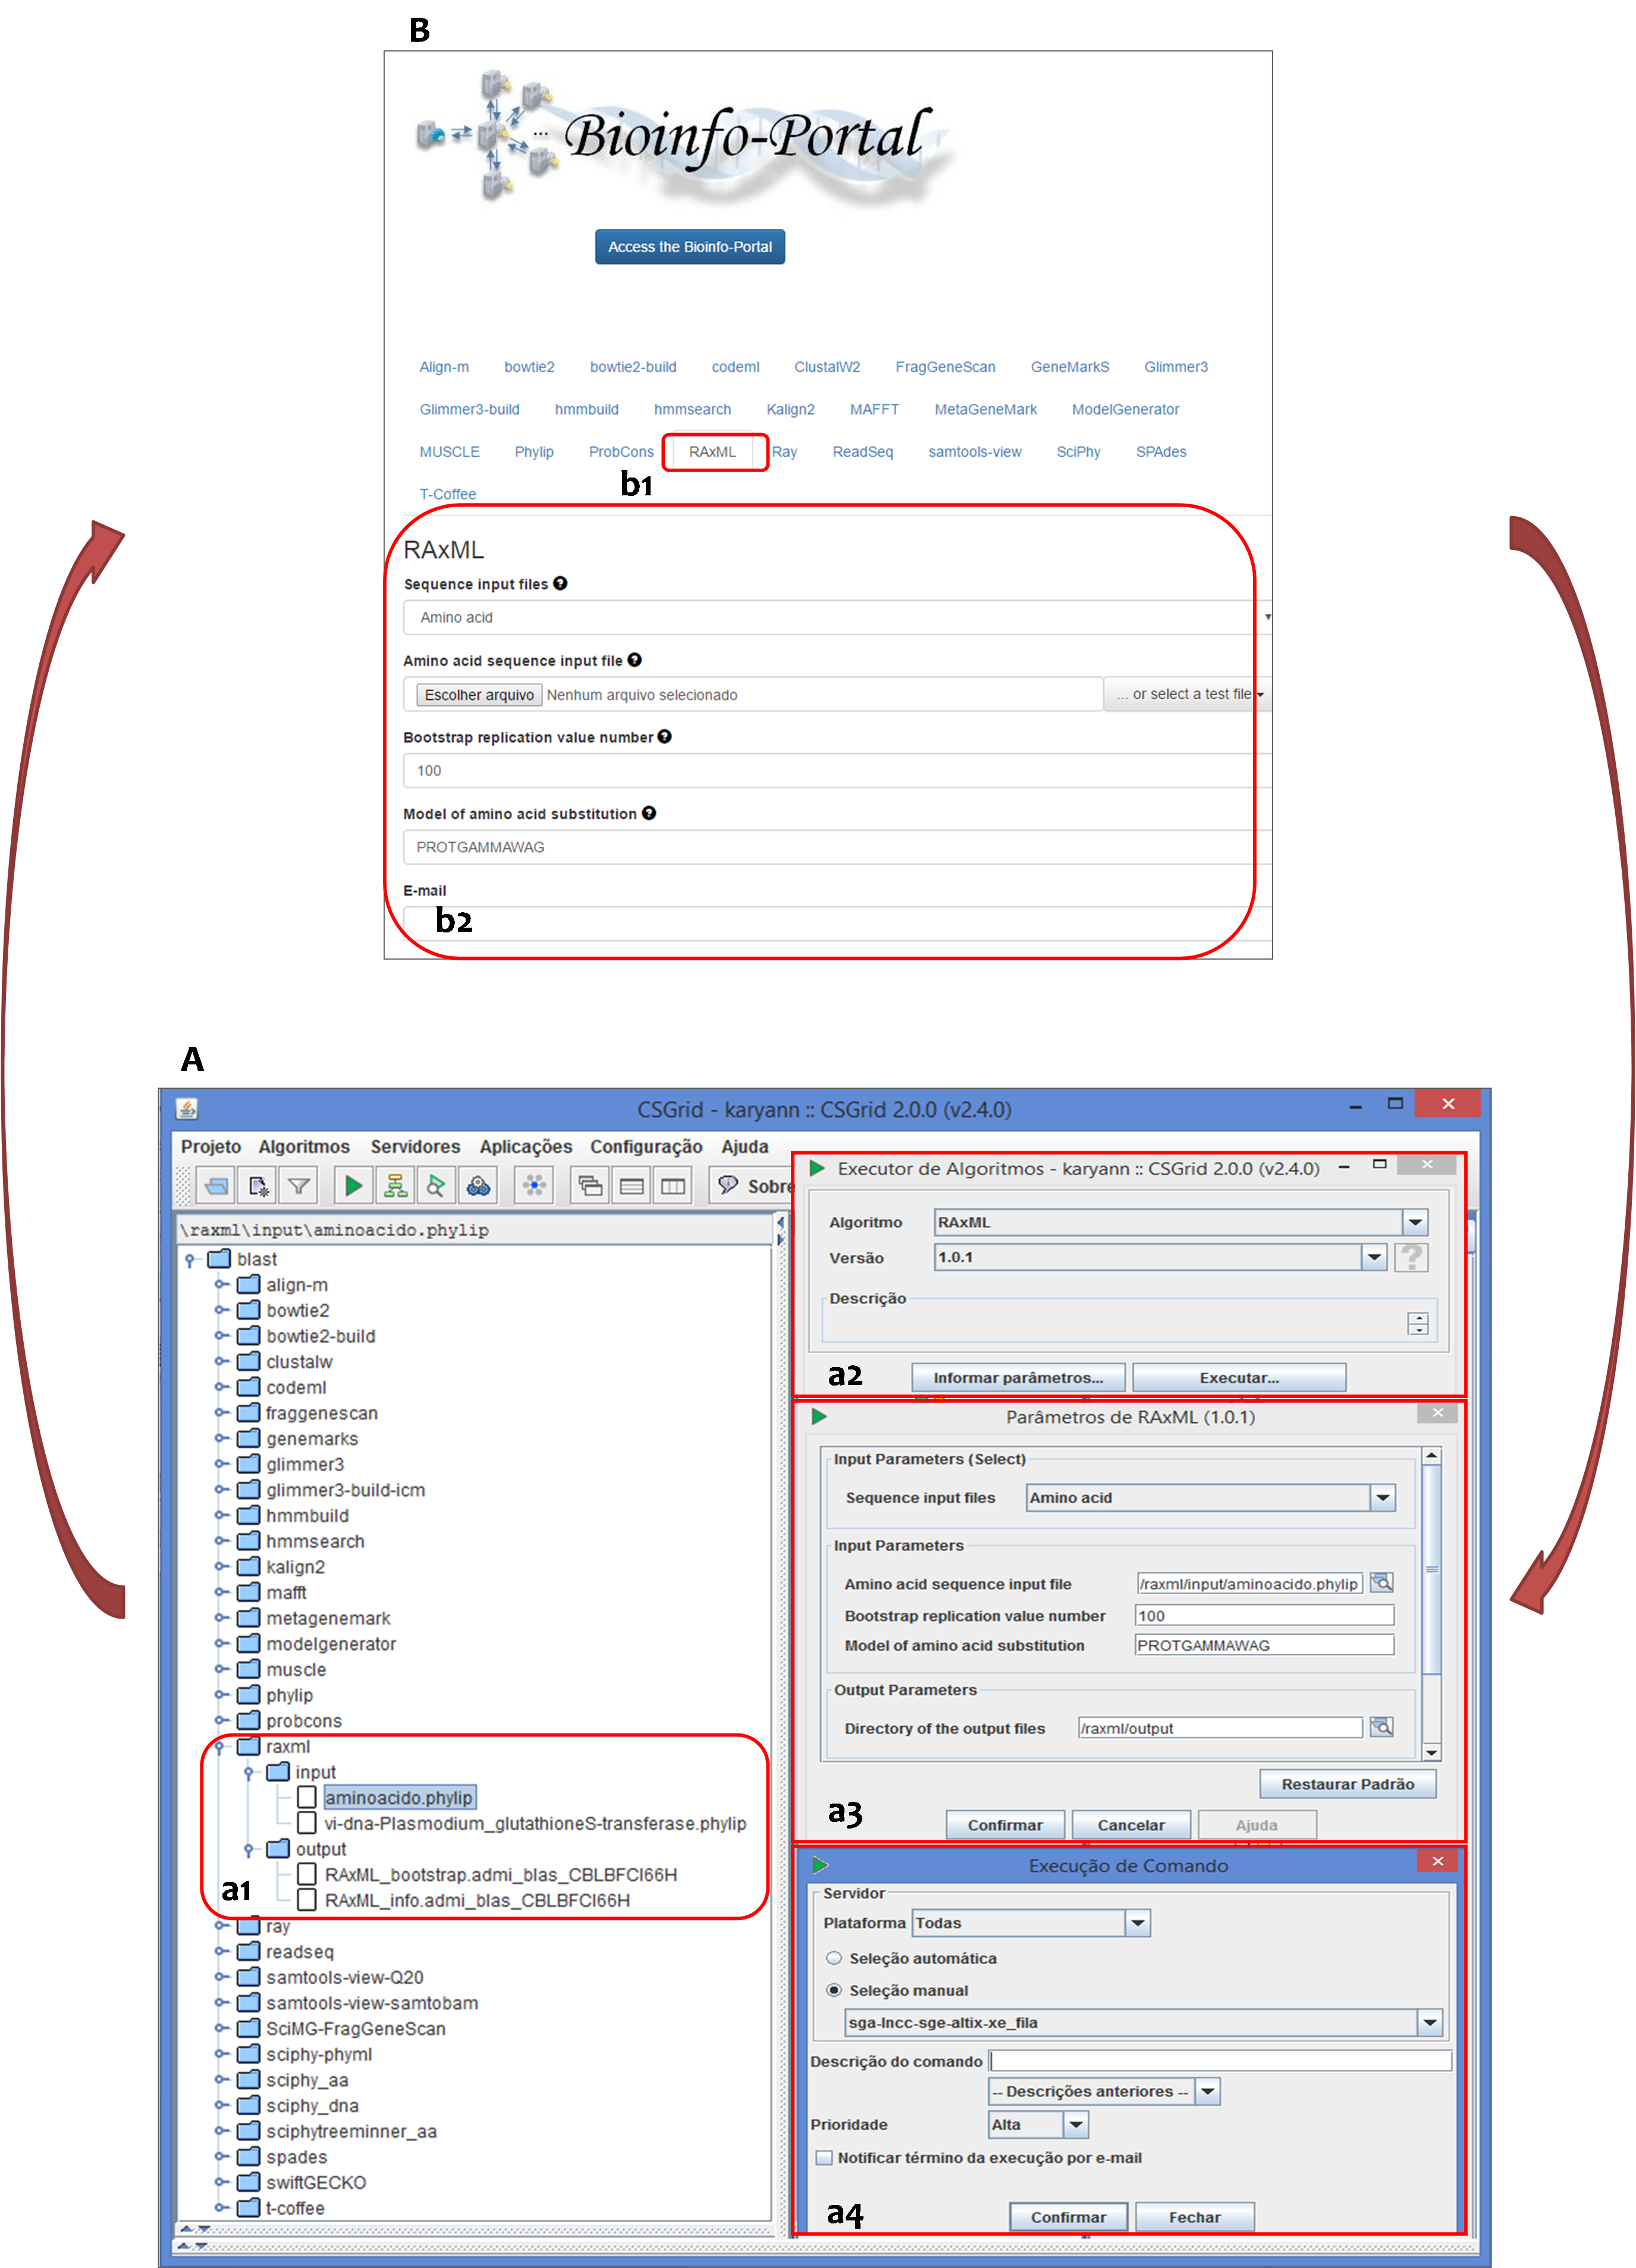
\includegraphics[height=10cm]{imgs/raxmlalgorithm.png}
	\vspace{-7px}
\caption{The Algorithm of the software ~\raxml at the \system front-end.} \label{fig:raxmlalgorithm}
\end{center}
\end{figure}

\vspace{5px}
\noindent
\underline{\textbf{\sci}} is a bioinformatics workflow that aims at constructing ML phylogenetics trees and takes as input data sequences of DNA, RNA, or amino acid. \sci is managed with the SWfMS SciCumulus and its execution is computationally intensive. Figure~\ref{fig:sciphyworkflow} illustrates the \sci workflow, which essentially consists of three sequential activities followed by two concurrent activities, all implemented by black-box and external programs.
The pipeline can be summarized by the following activities:
\textit{(i)}~multiple sequence alignment, implemented by the MAFFT program, 
\textit{(ii)}~alignment format conversion, conducted through the ReadSeq program, 
\textit{(iii)}~best evolutionary model election, carried out by the ModelGenerator program, 
\textit{(iv)}~phylogenetic tree construction, implemented by the RAxML program. 
Since each one of these activities performs a parameter sweep individually, they generate several independent tasks.

\begin{figure}[!t]
\begin{center}
	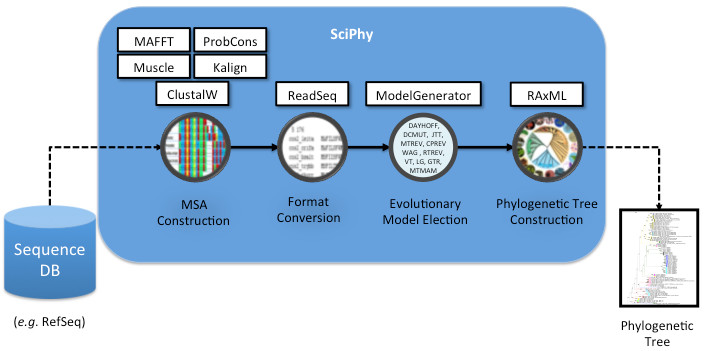
\includegraphics[height=7.7cm]{imgs/sciphyworkflow.png}
	\vspace{-7px}
\caption{The conceptual view of the workflow ~\sci with activities.} \label{fig:sciphyworkflow}
\end{center}
\end{figure}

SciCumulus’ provenance database stores domain data related to the workflow \sci. It is connected to the \system database at CSGrid, which provides the access to the information of other \system applications as well as to other services/portals at CSGrid/SINAPAD. As SciCumulus queries the provenance database at runtime, the Web interface of \system automatically will report messages of the \sci execution status \textit{e.g.} which activity is finished or if any error is presented. 
Figure~\ref{fig:sciphyalgorithm} shows the \sci Web interface at Bioinfo-Portal. This layout is automatically generated based on the configuration scripts config.xml (Additional file 4), execute.sh (Additional file 7), and prescript.sh (Additional file 8). The input arguments required by \sci at \system are one input file (\textit{e.g.} alignment in FASTA format), one selection option for input file type (\textit{e.g.} amino acid), an e-mail address, and one directory for output files. 

\begin{figure}[!t]
\begin{center}
	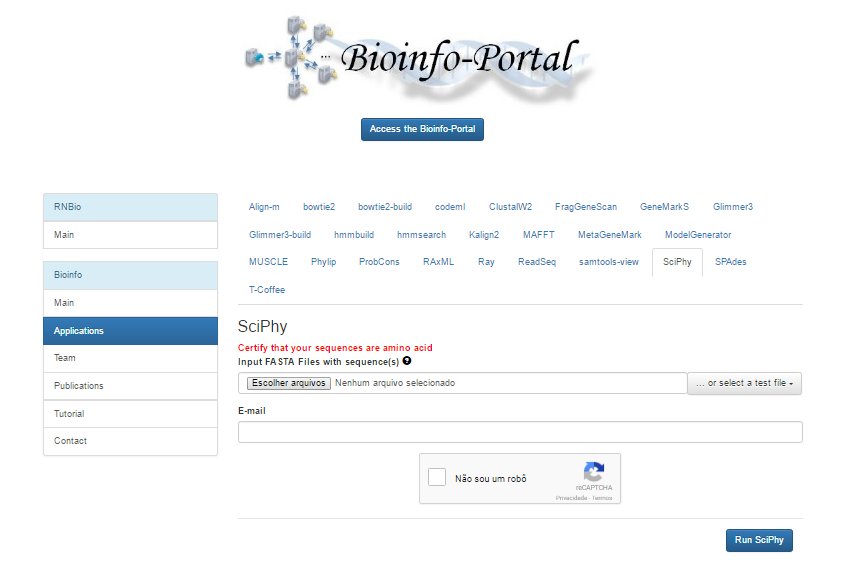
\includegraphics[height=8.7cm]{imgs/sciphyalgorithm.png}
	\vspace{-7px}
\caption{The Algorithm of the software ~\sci at the \system front-end.} \label{fig:sciphyalgorithm}
\end{center}
\end{figure}

\vspace{5px}
\noindent
\underline{\textbf{\swift}} is the workflow that maps the application GECKO {REF} using the SWfMS Swift which provides task-level parallelization and provenance data tracking. GECKO was designed to identify collections of high-scoring segment pairs (HSPs) by genome comparisons.Figure \ref{fig:swiftgeckoworkflow} describes the three modules of the workflow \swift that is composed at total for ten activities:
\textit{(i)}~Dictionary Calculation, which created dictionaries for the sequence input data; it is composed of activities 1-4,
\textit{(ii)}~high-scoring segment pairs (HSP) Detection, which detects hits used to identify the HSP locations; it is composed activities 5-9, in green boxes, and
\textit{(iii)}~Post-processing, which performs statistical calculations and functional annotations; it is composed by the activity 10, in the orange box.
\vspace{5px}

\begin{figure}[!t]
\begin{center}
	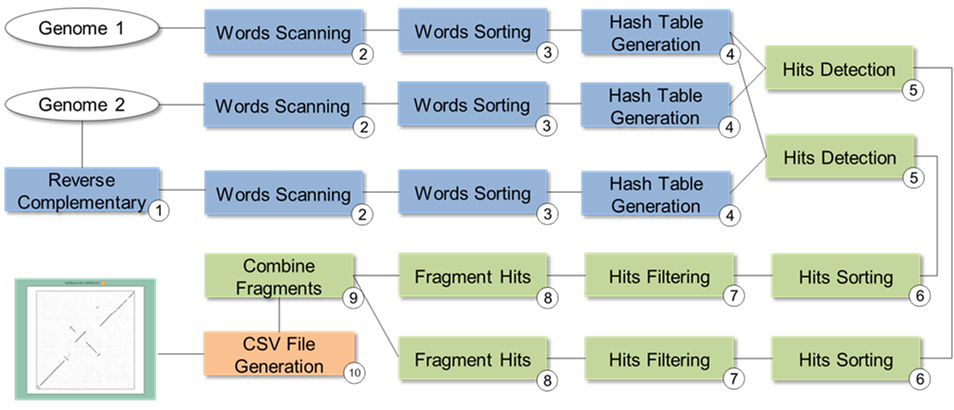
\includegraphics[height=6.7cm]{imgs/swiftgeckoworkflow.png}
	\vspace{-7px}
\caption{The conceptual view of the workflow ~\swift with activities.} \label{fig:swiftgeckoworkflow}
\end{center}
\end{figure}

The provenance database of \swift stores the provenance data information as the TET and the scientific domain data information. By querying the provenance database of Swift, specialists can infer about the evolutionary and taxonomic relationship of genomes based on the number of fragments, also crossing with computational information of CPU consumed. The input arguments required by \swift at \system, are one input file (genomes in FASTA format), one selection option for GECKO parameters (length, similarity, word length, FixedL), and an e-mail.
Figure~\ref{fig:swiftgeckoworkflow} shows the \swift Web interface at \system and the input arguments required are one input file \textit{i.e.} the genomes, the parameters of GECKO and the user's e-mail for returning results.

\begin{figure}[!t]
\begin{center}
	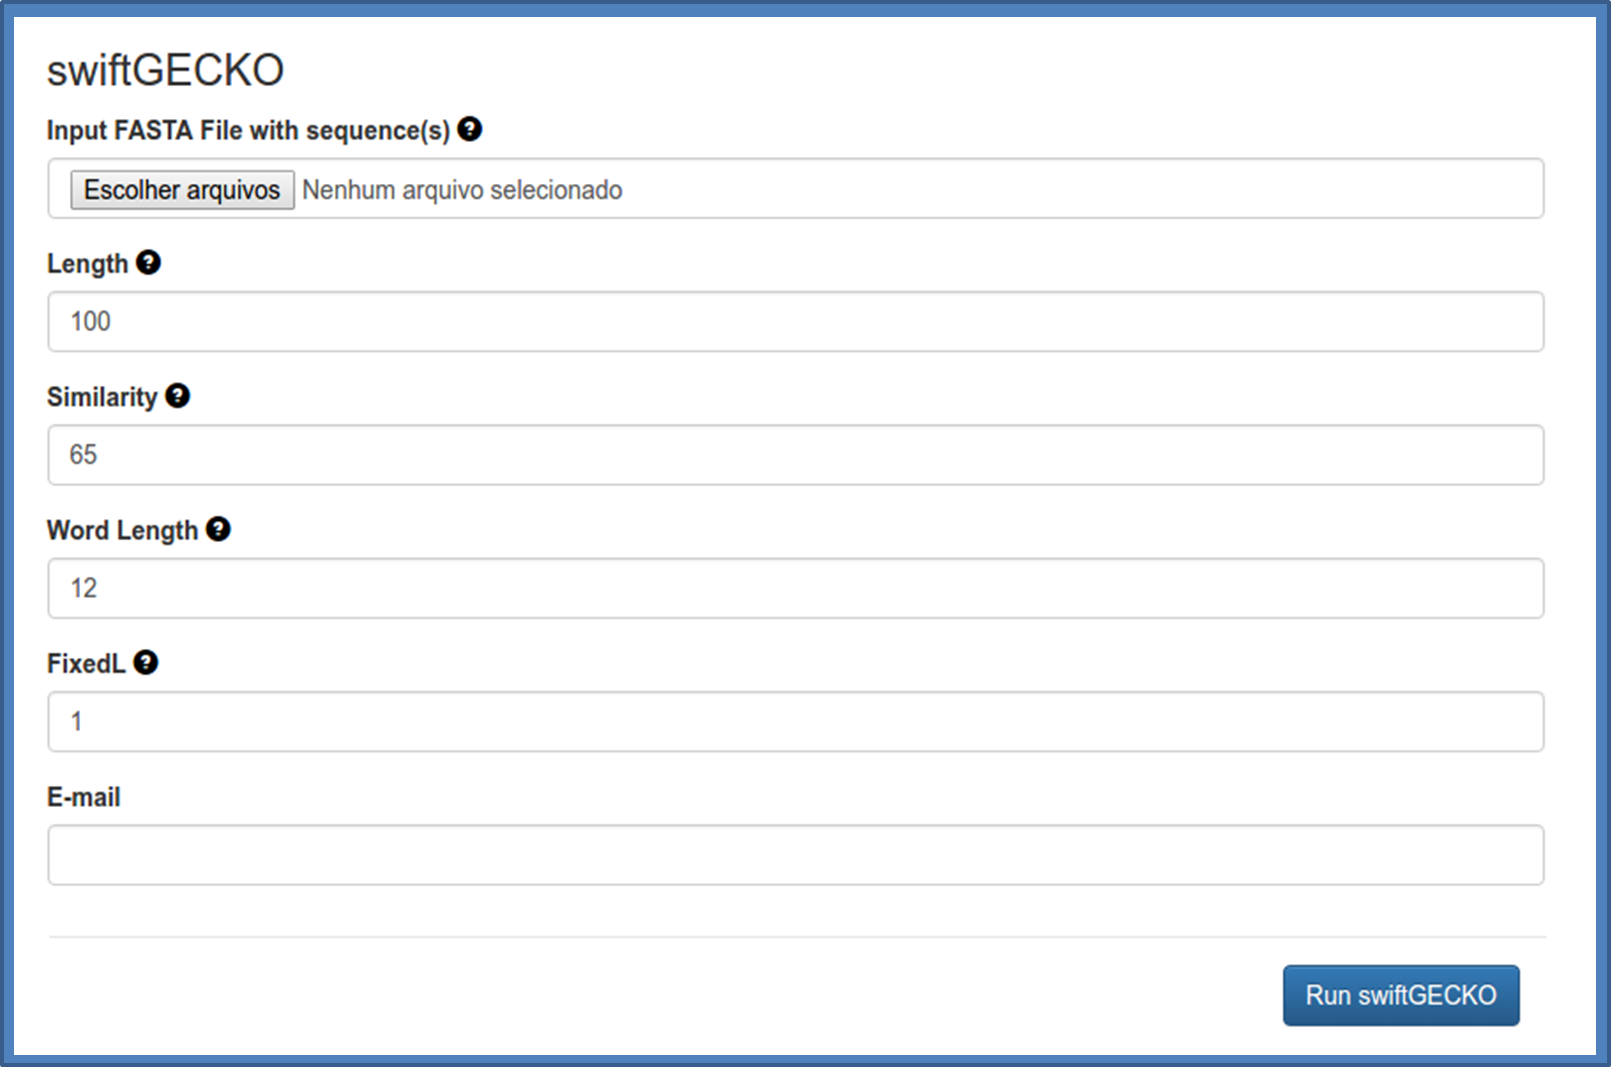
\includegraphics[height=7.7cm]{imgs/swiftgeckoalgorithm.png}
	\vspace{-7px}
\caption{The Algorithm of the software ~\swift at the \system front-end.} \label{fig:swiftgeckoalgorithm}
\end{center}
\end{figure}

\subsection{Experimental Data and Setup} \label{expsetup}
The experiments of ~\raxml, ~\sci, and ~\swift were executed in the cluster Altix ICE\footnote{\url{http://www.lncc.br/ice/}} and supercomputer SDumont\footnote{\url{http://sdumont.lncc.br/}}. Altix consists of 25 diskless machines (execution nodes), each node is given by an SGI ICE 8400 server with 2 Intel Xeon X5650 2.67GHz Hexa Core processors (totaling 12 cores) and 48 GB DDR3 DIMMs of memory. The cluster has one login node with a gross storage capacity of 5TB. SDumont consists of 16 TB RAM, storage totaling 1,7 PetaBytes (Seagate 1.5 Buster), 10.692 cores, 1.1 PetaFlops, Intel Xeon E5-2695v2, 30 MB cache, 12 cores – 3.2 GHz.

\underline{\textbf{\raxml}} experiment data is formed by amino acid superalignments in format PHYLIP. Table~\ref{tab:superalignments} presents the features of the superalignments used as input data for the execution of \raxml. The eight superalignment files were categorized as Large (D1, D2), Medium (D3, D4, D7, D8), and Small (D5, D6). This classification was based on the features of the alignment sequences as the Number of Taxa, Number of Amino Acid, and Size in KB. For example, the input file D5 has a size of 79 KB and it is formed of 31 concatenated universal orthologous (UO) genes from 12 protozoan genomes. \underline{\textbf{\sci}} experiment data are input file of amino acid sequences of 200 multi-fasta alignments in FASTA format. The biological sequences used for constructing phylogenetic trees are orthologous genes of 12 protozoan genomes. \underline{\textbf{\swift}} experiment data are input file of amino acid sequences of eight mammalian genomes in FASTA format. 

\begin{table}[!t]
\centering
\caption{Comparison of alternatives for provenance support in Spark.}
\label{tab:superalignments}
\resizebox{\textwidth}{!}{\begin{tabular}{|l|p{2.2cm}|p{2.2cm}|p{2.2cm}|p{2.2cm}|p{2.2cm}|p{2.2cm}|}
\hline
\multirow{2}{*}{} & \multicolumn{4}{c|}{\textbf{Features}} \\ \cline{2-5} 
                      & \textbf{Category} & \textbf{Number of Taxa}  & \textbf{Number of Amino Acid}  & \textbf{Size in KB}     \\ \hline\hline
                      
\textbf{Superalignment D1}    
& Large   & 74   &  21,260   &  2,091   \\ \hline
\textbf{Superalignment D2}      
& Large   & 74   &  12,807   &  1,260   \\ \hline
\textbf{Superalignment D3}      
& Medium   & 26   &  22,906   &  792   \\ \hline
\textbf{Superalignment D4}       
& Medium   & 26   &  16,068   &  553   \\ \hline
\textbf{Superalignment D5}     
& Small   & 12   &  4,941   &  79   \\ \hline
\textbf{Superalignment D6}     
& Small   & 12   &  4,481   &  72   \\ \hline
\textbf{Superalignment D7}     
& Medium   & 36   &  3,490   &  168   \\ \hline
\textbf{Superalignment D8}     
& Medium   & 36   &  3,270   &  157   \\ \hline
\end{tabular}}
\end{table}

\subsection{\system settings: the architecture of the science gateway}

CSGrid provides the central infrastructure for developing the Algorithms and managing executions using the computational resources of SINAPAD. Each Algorithm presents scripts of configuration (“.xml”) and execution (“.sh”), which are modified/implemented following the requirements of the applications or computational resources. The main scripts are \texttt{portal.xml} that configures the main web interface of \system; \texttt{config.xml} that configures the parameters used by each Algorithm; \texttt{execute.sh} that executes the Algorithm based on the parameters of \texttt{config.xml}; and \texttt{prescript.sh} that presents the parameters to configure the environment for the computational resources. Figure~\ref{fig:raxmlmanagement} presents the structure of CSGrid for the Algorithm ~\raxml, the scripts, and the available computational resources.

\begin{figure}[!t]
\begin{center}
	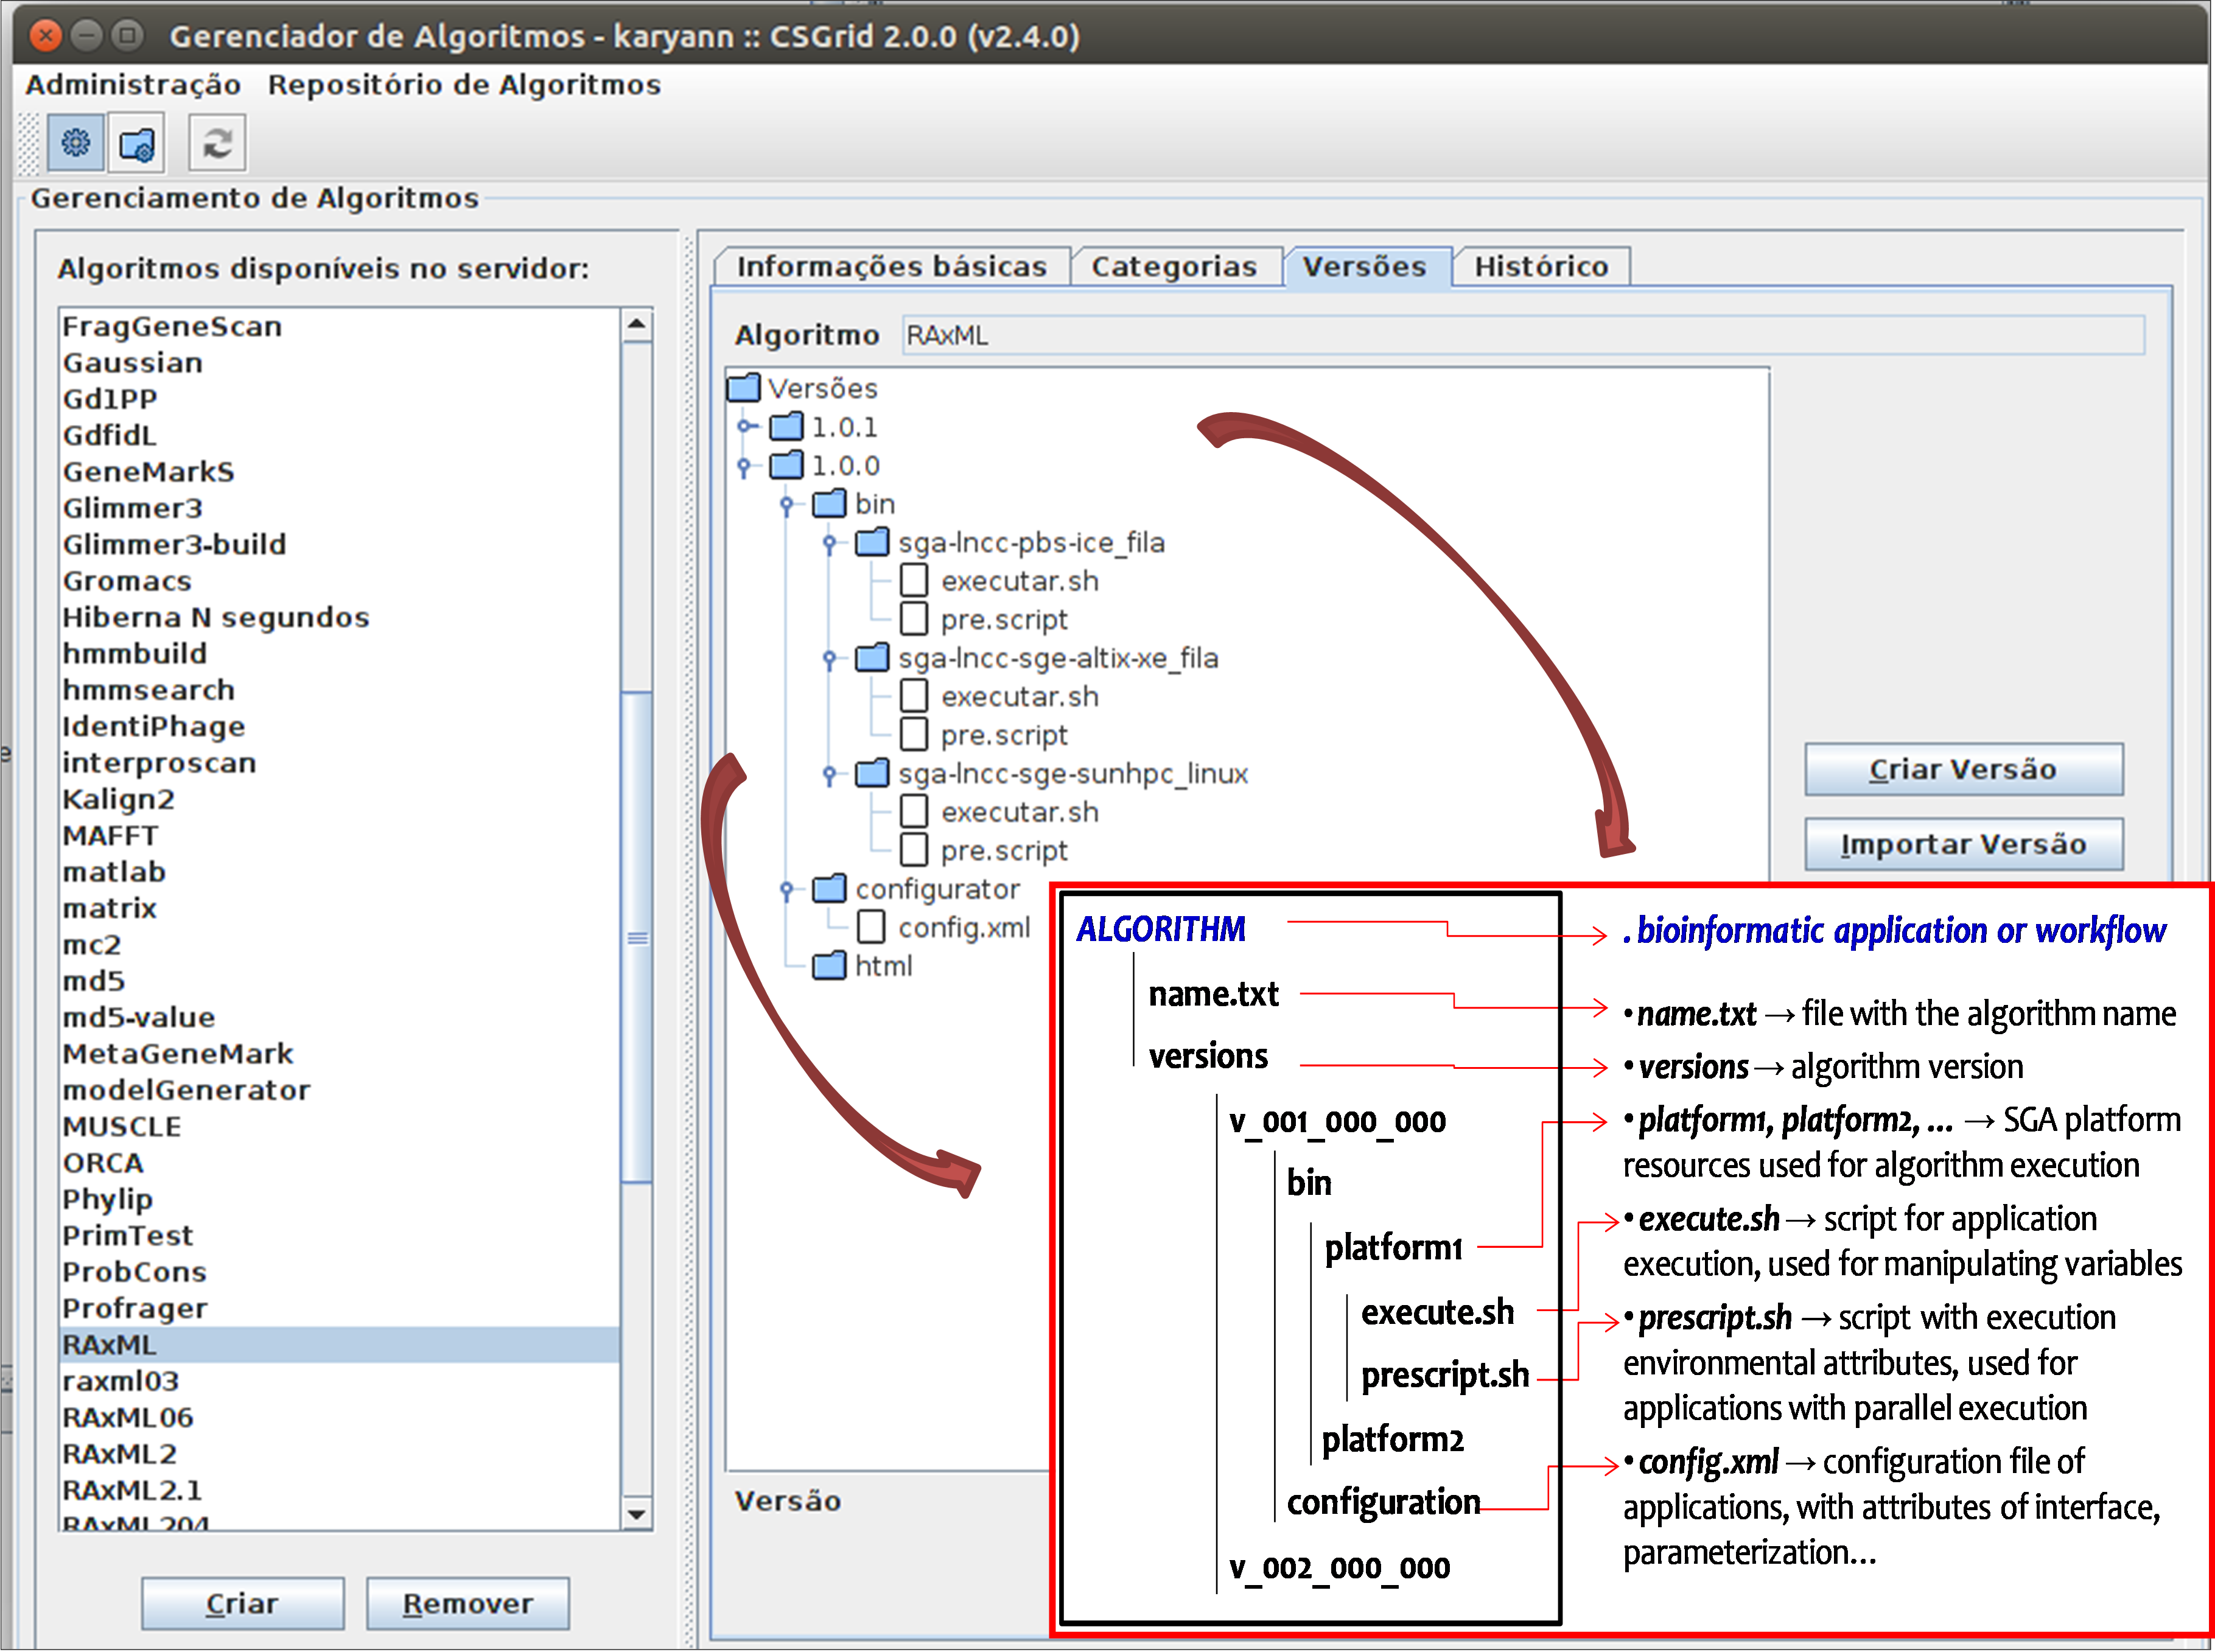
\includegraphics[height=8.7cm]{imgs/raxmlmanagement.png}
	\vspace{-7px}
\caption{The management of the Algorithm ~\raxml at the CSGrid of the \system front-end.} \label{fig:raxmlmanagement}
\end{center}
\end{figure}

\underline{\textbf{portal.xml}} connects the web interface of \system to the Project area of the Algorithms. CSGrid defines which Algorithm will be executed by the gateway. The user must select the Algorithm; then, the web interface is dynamically built in the gateway and provides the fields of input/output and parameters that need to be filled by the user. The \texttt{portal.xml} allows that multiple versions of the same Algorithm be available at the gateway (XML attribute multiple-versions); then users can execute several versions of the applications. The final excerpt of Figure~\ref{fig:portalxmlcode} presents an example of a configuration script invocation, whose parameters are required for the processing of the Algorithms \raxml and \sci in \system. 

 \begin{figure}[!t]
 \begin{lstlisting}[style=myScalastyle]
 // The script portal.xml for RaXML and SciPhy
1    <portal-config multiple-versions="true" resource-choice="true" auto-generate="true">
2            ...
3            <acronym-name>Bioinfo</acronym-name>
4            <full-name>Bioinfo-Portal Gateway</full-name>
5            <csgrid-project-name> Bioinfo </csgrid-project-name>
6            <algorithms-config>
7                    <algorithm>
8                           <name>RAxML</name>
9                           <default-version>1.0.0</default-version>
10                   </algorithm>
11                   <algorithm>
12                           <name>SciPhy</name>
13                           <default-version>1.0.0</default-version>
14                   </algorithm>
15           </algorithms-config>
16           ...
17   </portal-config>

\end{lstlisting}
\vspace{-10px}
\caption{Implementation of the configuration script \texttt{portal.xml} for the invocations of Algorithms \raxml and \sci in \system.}
\label{fig:portalxmlcode}
\end{figure}

\underline{\textbf{config.xml}} describes the input/output arguments required by each Algorithm. It is similar in purpose to the files of the JSON Service Description Language (JSDL) of the middleware UNICORE \cite{ref10.1007/11508380_38} and the Common Tool Description (CTD) of the OpenMS library. Nevertheless, \texttt{config.xml} provides more details about how the arguments of the Algorithm can be rendered in a user interface \textit{e.g.} to the conditional attributes: “for the Algorithm RAxML, the fields A (amino acid type) and B (nucleotide type) are mutually exclusive”. These attributes allow users to hide/disable field(s) at the web interface determined by one specific value of the flag. The \texttt{config.xml} is used by CSGrid for dynamically assembling the web interfaces and by the OpenDreams service for invocating the commands of scripts that reify the Algorithm in the underlying computational resources. The final excerpt of Figure~\ref{fig:configxmlcoderaxml} presents an example of the invocation of a configuration script and whose parameters are required for processing the Algorithm \raxml in \system. Figure~\ref{fig:configxmlcoderaxml} presents the example for invocating the Algorithm \sci in \system. 

 \begin{figure}[!t]
 \begin{lstlisting}[style=myScalastyle]
 // The script config.xml for RaXML
1    <?xml version='1.0' encoding='UTF-8'?>
2    <algorithm command="execute.sh" capture_code_ouput="yes" provide_identifier="yes">
3        <format_command>$NAME_PARAMETER=$VALUE_PARAMETER </format_command>
4        <group label='Input Parameters (Select)'>
5            <enum name="RAXML_INPUTTYPES" label="Input files" clue="Select file(s)"standard="dna">
6                <item_enum id="aa" label="Amino acid" value="aa" clue="Provide amino acid input file"/>
7                <item_enum id="dna" label="Nucleotide" value="dna" clue="Provide nucleotide input file"/>
8            </enum>
9        </group>
10      <group label="Input Parameters">
11          <entire name="numCPU"
              label="CPUs number"
              minimum="1"
              maximum="16"
              clue="Set the number of threads to allocate (min 1 - max 16)"
              standard="16"
              optional="true"/>
12          <file_input name="RAXML_INPUT_AA"
              label='Amino acid sequence input file'
              clue='Select or upload the amino acid sequence input file'/>
13          <file_input name="RAXML_INPUT_DNA"
              label='Nucleotide sequence input file'
              clue='Select or upload the right sequence input file'/>
14          <entire name="RAXML_BOOTSTRAP"
              label="Bootstrap replication value number"
              minimum="1" 
              maximum="2000"
              clue ="Set the number of replication for bootstrap (default 100)"
              standard="100"
              optional="true"/>
15          <text name="RAXML_MODEL_DNA"
              label="Model of nucleotide substitution"
              clue="Model of nucleotide substitution"
              standard="GTRGAMMA"
              optional="true"/>
16          <text name="RAXML_MODEL_AA"
              label="Model of amino acid substitution"
              clue="Model of amino acid substitution"
              standard="PROTGAMMAWAG"
              optional="true"/>
17      </group>
18      <group label='Output Parameters'>
19          <file_output name="RAXML_OUTPUT" 
              label="Directory of the output files" 
              clue="Select the output directory where the result files will be placed" 
              category="directory"/>
20      </group>
21      <display>
22          <parameter name="RAXML_INPUT_DNA"/>
23          <parameter name="RAXML_MODEL_DNA"/>
24          <condition parameter="RAXML_INPUTTYPES" value="dna"/>
25      </display>
26      <display>
27          <parameter name="RAXML_INPUT_AA"/>
28          <parameter name="RAXML_MODEL_AA"/>
29          <condition parameter="RAXML_INPUTTYPES" value="aa"/>
30      </display>
31  </algorithm>
\end{lstlisting}
\vspace{-10px}
\caption{Implementation of the configuration script \texttt{config.xml} for the invocations of Algorithm \raxml in \system.}
\label{fig:configxmlcoderaxml}
\end{figure}

 \begin{figure}[!t]
 \begin{lstlisting}[style=myScalastyle]
 // The script config.xml for SciPhy
1    <?xml version='1.0' encoding='UTF-8'?>
2    <algorithm command="execute.sh" capture_code_ouput="yes" provide_identifier="yes">
3        <format_command>$NAME_PARAMETER=$VALUE_PARAMETER </format_command>
4        <group label="Input Parameters">
5          <file_input name=" SciPhy_INPUT "
              label="Input directory of FASTA file(s)"
              clue="Select or upload the input fasta file(s), not exceed 10 files or 10 Mb in size"
              category="directory"/>
6      </group>
7    <group label='Output Parameters'>
8          <file_output name=" SciPhy_OUTPUT" 
              label="Directory of the output files" 
              clue="Select the output directory where the result files will be placed" 
              category="directory"/>
9      </group>
10  </algorithm>

\end{lstlisting}
\vspace{-10px}
\caption{Implementation of the configuration script \texttt{config.xml} for the invocations of Algorithm \sci in \system.}
\label{fig:configxmlcodesciphy}
\end{figure}

\underline{\textbf{execute.sh}} describes the specific arguments used for the execution of the Algorithms belonging to each one of the bioinformatics applications. The arguments or parameters can be extracted from the command line used to execute the applications. The final excerpt of Figure~\ref{fig:executeshcoderaxml} presents an example for the invocation of a execution script and whose parameters are required for the processing of the Algorithm \raxml in \system. 

 \begin{figure}[!t]
 \begin{lstlisting}[style=myScalastyle]
 // The script execute.sh for RAxML
1    #!/bin/bash
2    . ~/setclasspath.sh
3    . /hpc/modulos/bash/openmpi-1.8.5-gcc47.sh
4    function parseArgs {
5        for arg in $* ; do
6            typeset name=`echo $arg | sed "s/=.*//"`
7            typeset value=`echo $arg | sed "s/.*=//"`
8            export $name=$value
9        done
10  }

 // CSGrid Arguments
11  parseArgs $*
12  echo "Id SGE: "$JOB_ID, $RAXML_INPUTTYPES, $RAXML_INPUT_DNA, $RAXML_INPUT_AA, $RAXML_BOOTSTRAP, $RAXML_MODEL_AA, $RAXML_MODEL_DNA, $RAXML_OUTPUT
13  cmdId=`echo $cmdId | sed 's/\(.*\)\@\(.*\)\.\(.*\)/\1_\2_\3/'`

 // Execute RAxML
14  cd $RAXML_OUTPUT
15  numCPU=$NSLOTS
16  COMMAND="/usr/bin/time -f "%e" -o ${RAXML_OUTPUT}/.time.log 2  $ALGORITHMS_THIRD_DIR/RAxML/versions/v_001_000_000/RAxML/standard-RAxML-master/raxmlHPC-MPI-SSE3"
17  COMMANDmpi="/usr/bin/time -f "%e" -o ${RAXML_OUTPUT}/.time.log mpirun -np $numCPU -hostfile $TMPDIR/hostfile $ALGORITHMS_THIRD_DIR/RAxML/versions/v_001_000_000/RAxML/standard-RAxML-master/raxmlHPC-MPI-SSE3"
18  if [ "$RAXML_INPUTTYPES" == "dna" ]
19  then
 // Best tree
20      EXEC1="$COMMAND -m $RAXML_MODEL_DNA -p 112233 -s $RAXML_INPUT_DNA -n $cmdId.best -c 4 -f d"
21      $EXEC1
 // Bootstrap
22      EXEC2="$COMMAND -m $RAXML_MODEL_DNA -p 112233 -s $RAXML_INPUT_DNA -b 223344 -# $RAXML_BOOTSTRAP -n $cmdId.bootreps -c 4 -f d"
23      $EXEC2
 // Consense
24      EXEC3="$COMMAND -m $RAXML_MODEL_DNA -s $RAXML_INPUT_DNA -f b -t RAxML_bestTree.$cmdId.best -z RAxML_bootstrap.$cmdId.bootreps -n $cmdId.bestML.bootstrap"
$EXEC3
25  fi
26  if [ "$RAXML_INPUTTYPES" == "aa" ]
27  then
 // Best tree
28      EXEC1="$COMMAND -m $RAXML_MODEL_AA -p 112233 -s $RAXML_INPUT_AA -n $cmdId.best -c 4 -f d"
29      $EXEC1
 // Bootstrap
30      EXEC2="$COMMAND -m $RAXML_MODEL_AA -p 112233 -s $RAXML_INPUT_AA -b 223344 -# $RAXML_BOOTSTRAP -n $cmdId.bootreps -c 4 -f d"
31      $EXEC2
 // Consense
32      EXEC3="$COMMAND -m $RAXML_MODEL_AA -s $RAXML_INPUT_AA -f b -t RAxML_bestTree.$cmdId.best -z RAxML_bootstrap.$cmdId.bootreps -n $cmdId.bestML.bootstrap"
33      $EXEC3
34  fi

 // $COMMAND
35  if [ $? != 0 ]
36   then
37      echo "RAxML returned an error."
38      exit 1
39  fi
\end{lstlisting}
\vspace{-10px}
\caption{Implementation of the configuration script \texttt{execute.sh} for the invocations of Algorithm \raxml in \system.}
\label{fig:executeshcoderaxml}
\end{figure}

\underline{\textbf{prescript.sh}} describes the arguments used for the invocation of the script of the configuration of the environment. The final excerpt of Figure~\ref{fig:prescriptshcoderaxml} presents an example for the invocation of the script of execution and whose parameters are required for the processing the Algorithm \raxml in \system. 

 \begin{figure}[!t]
 \begin{lstlisting}[style=myScalastyle]
 // The script prescript.sh for RAxML
1    #$ -N JOB_RAXML
2    #$ -cwd
3    #$ -V
4    #$ -pe mpi 16
5    #$ -l h_rt=216000
\end{lstlisting}
\vspace{-10px}
\caption{Implementation of the configuration script \texttt{prescript.sh} for the invocations of Algorithm \raxml in \system.}
\label{fig:prescriptshcoderaxml}
\end{figure}


\subsection{Performance on \system}
As the first \system evaluation, we measured the performance and scalability of executions of the applications \raxml, \sci, and \swift. Every experiment of applications was evaluated separately in order to highlight the impact of each feature individually. We executed all experiments of \system in SDumont clusters. Additionally, all executions provenance data were used as input information for executing machine learning analyses in order to determine the general features of application executions according to input size, software parameters, and efficiency that better offer requirements for optimizing the allocation of machines capacity for experiments.

\vspace{5px}
\noindent
\underline{\textbf{\raxml} Performance Analyses}

\textit{1) The total execution time of the versions of \raxml}. The \raxml HPC Serial was executed in one single core, \raxml PThreads in 12 cores, \raxml MPI in 120 cores, and \raxml Hybrid in 120 cores. The input file used in this experiment was the amino acid superalignment D5 in format PHYLIP, with a size of 79 KB and formed of 31 concatenated universal orthologous (UO) genes from 12 protozoan genomes. The parameters used for setting the \raxml versions are JTT as the evolutionary model, GAMMA as the rate of model heterogeneity, and 100 as the bootstrap value of replications. Figure~\ref{fig:raxmlTETD5} presents the Total Execution Time (TET) in minutes obtained after the execution of the versions of \raxml. The TET decreases using the parallel versions PThreads, MPI, and Hybrid of \raxml in comparison to the version \raxml HPC Serial and using the clusters of SDumont compared to Altix. For Altix, the \raxml MPI was the version that presented the best performance, with the TET reduced from 285,57 minutes (one single core) to 4.59 minutes (using 120 cores). For SDumont, the \raxml Hybrid was the version that presented the best performance, with the TET reduced from 161,29 minutes (using one single core) to 1.88 minutes (using 120 cores). 

\begin{figure}[!htb]
\centering
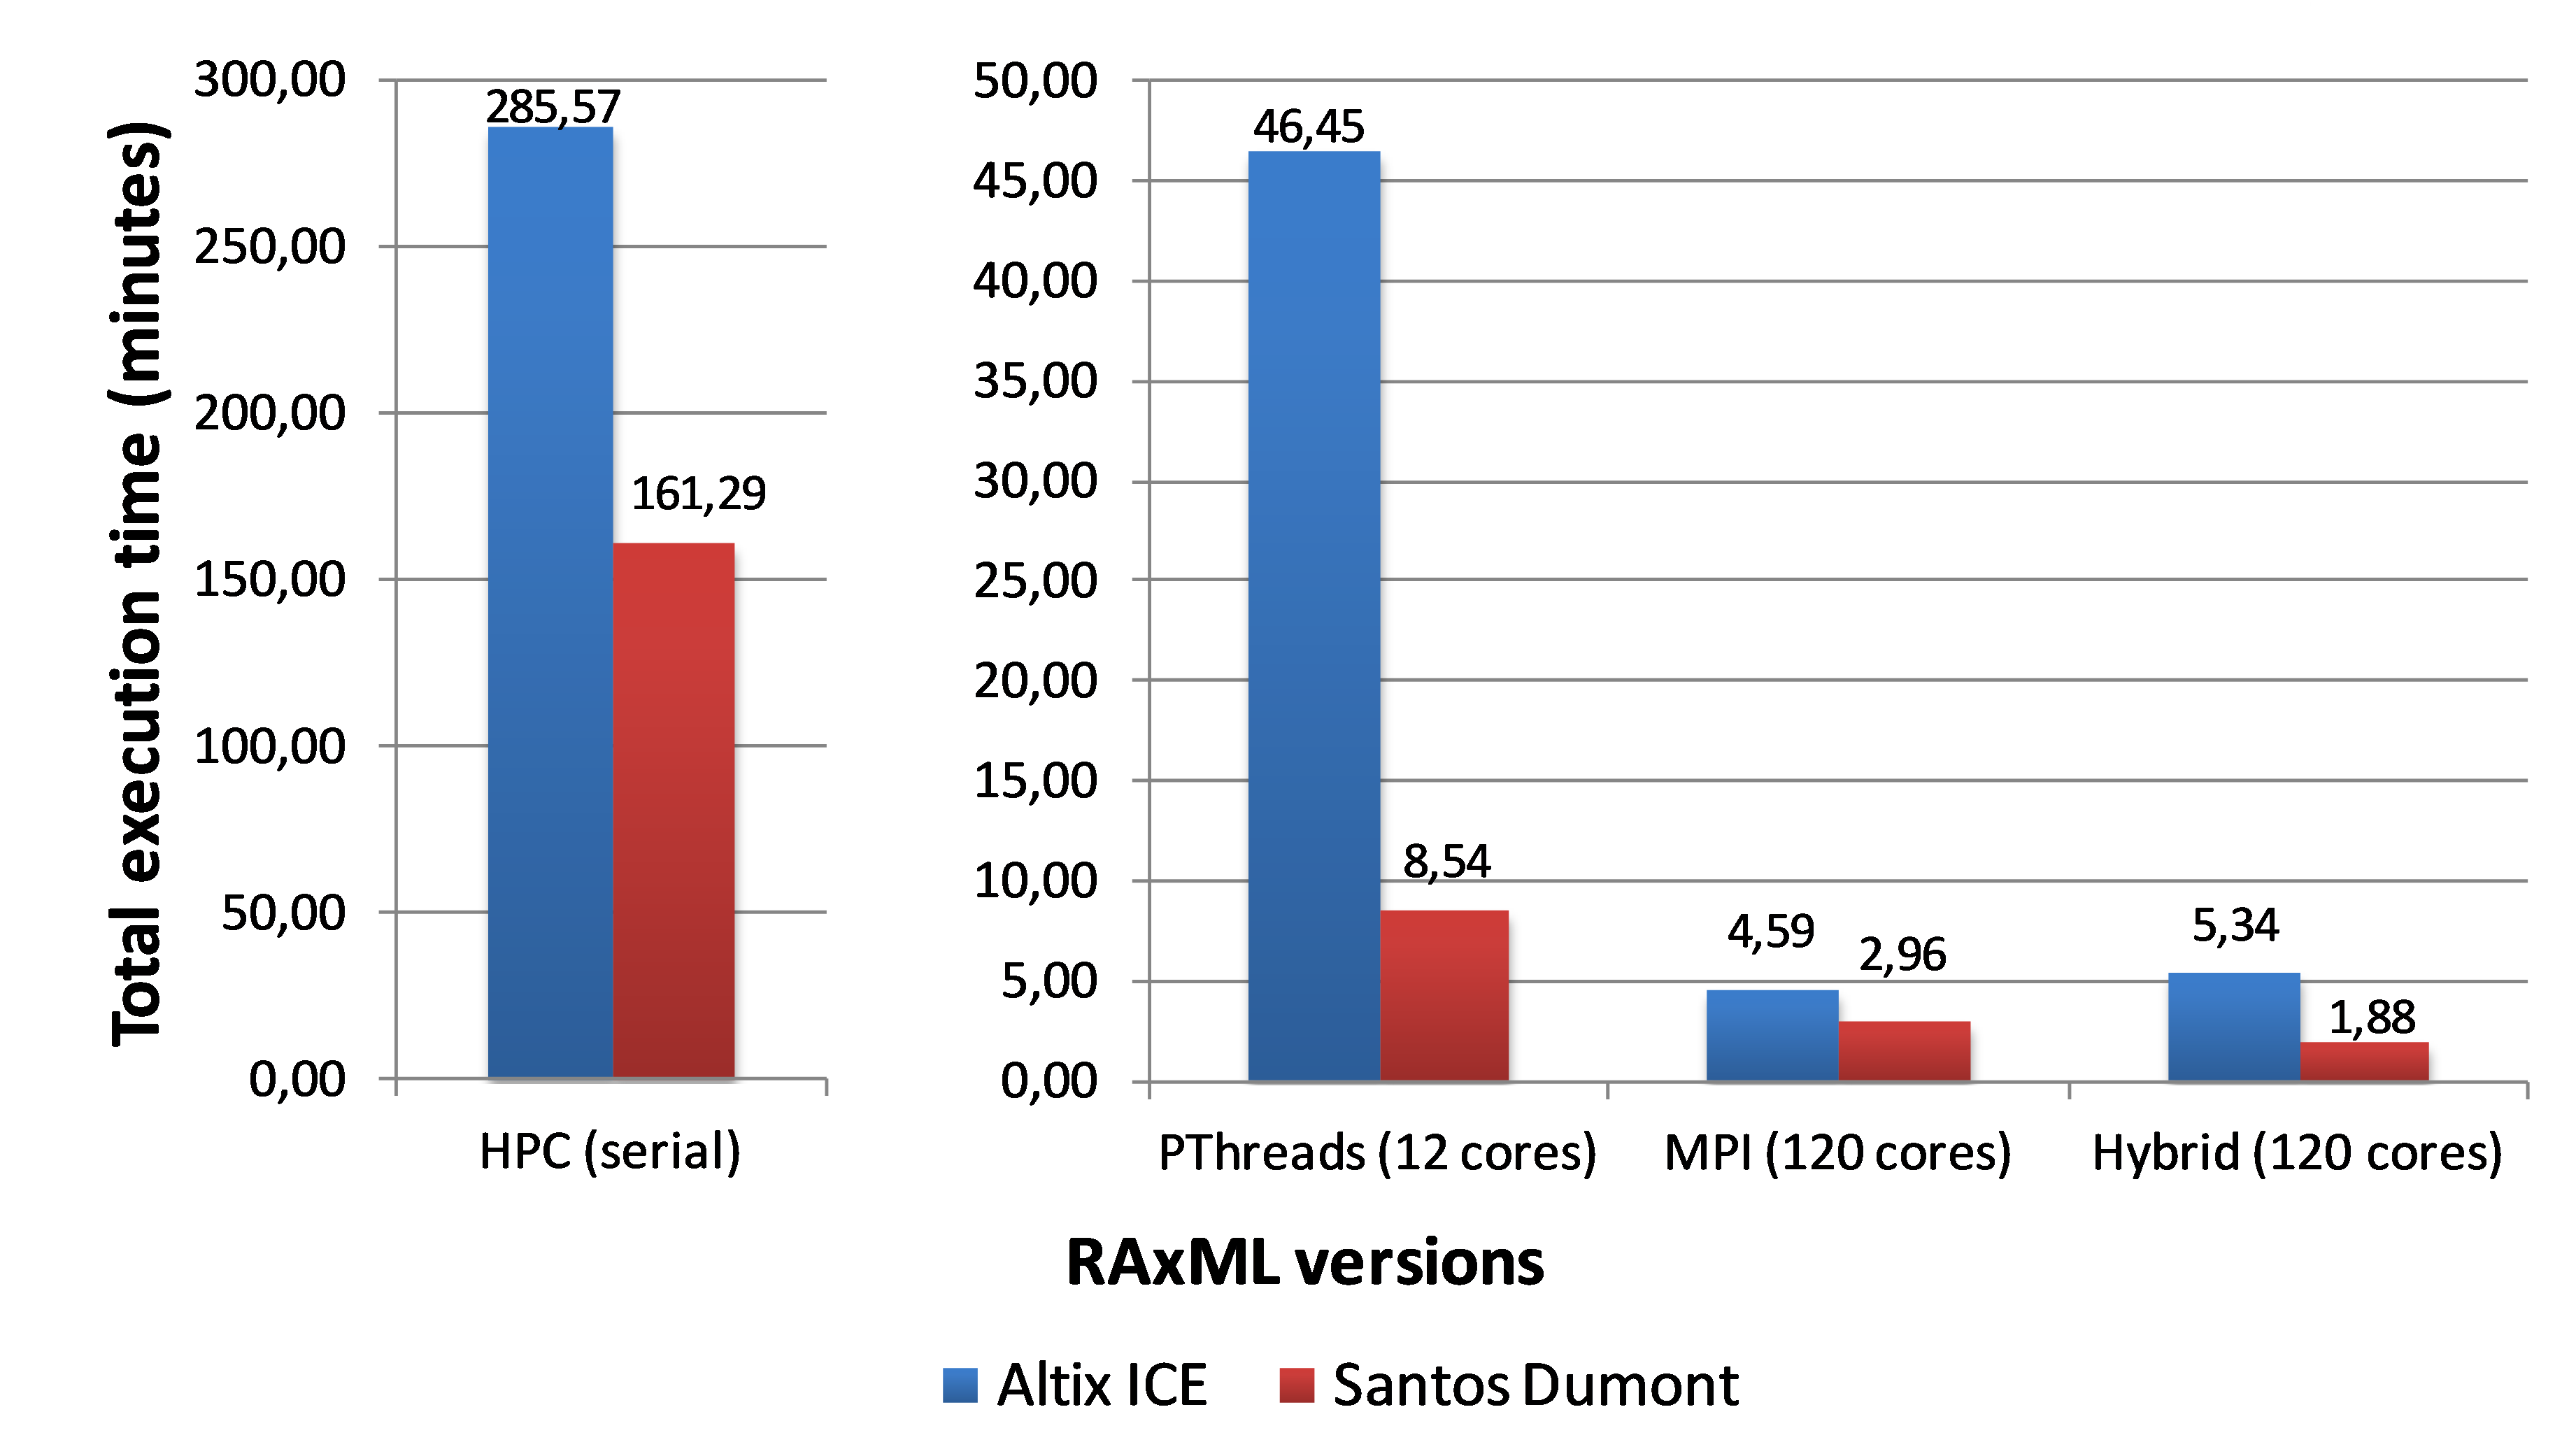
\includegraphics[width=0.6\textwidth]{imgs/raxmlTETD5.png}
\vspace{-12px}
\caption{\system performance (TET) results for \raxml in Altix and SDumont for the superalignment D5}
\label{fig:raxmlTETD5}
\end{figure}

\textit{2) The scalability of \raxml MPI (Altix) and \raxml Hybrid (SDumont)}. This experiment aims to evaluate the performance gains of the versions of \raxml that outperformed Altix (\raxml) and SDumont (\raxml Hybrid) according to the number of cores in minutes. The performance of \raxml was measured on a single processor machine (one core) to analyze the local optimization before scaling up the number of cores. After that, the performance and scalability of \raxml were measured using from 2 up to 120 cores. The superalignment used as input data is D5. Figure~\ref{fig:raxmlscalabilityD5} presents the scalability in minutes obtained after the execution of \raxml MPI in Altix and \raxml Hybrid in SDumont. The TET decreases, in both cases, as more cores were provided. \raxml Hybrid (SDumont) presented the best performance, the TET was reduced from 161.29 minutes (one single core) to 10.39 minutes (24 cores) and to 1.88 minutes (120 cores). Using one core, \raxml Hybrid at SDumont outperforms \raxml MPI at Altix; the TET was reduced from 285.57 minutes to 161.29 minutes.

\begin{figure}[!htb]
\centering
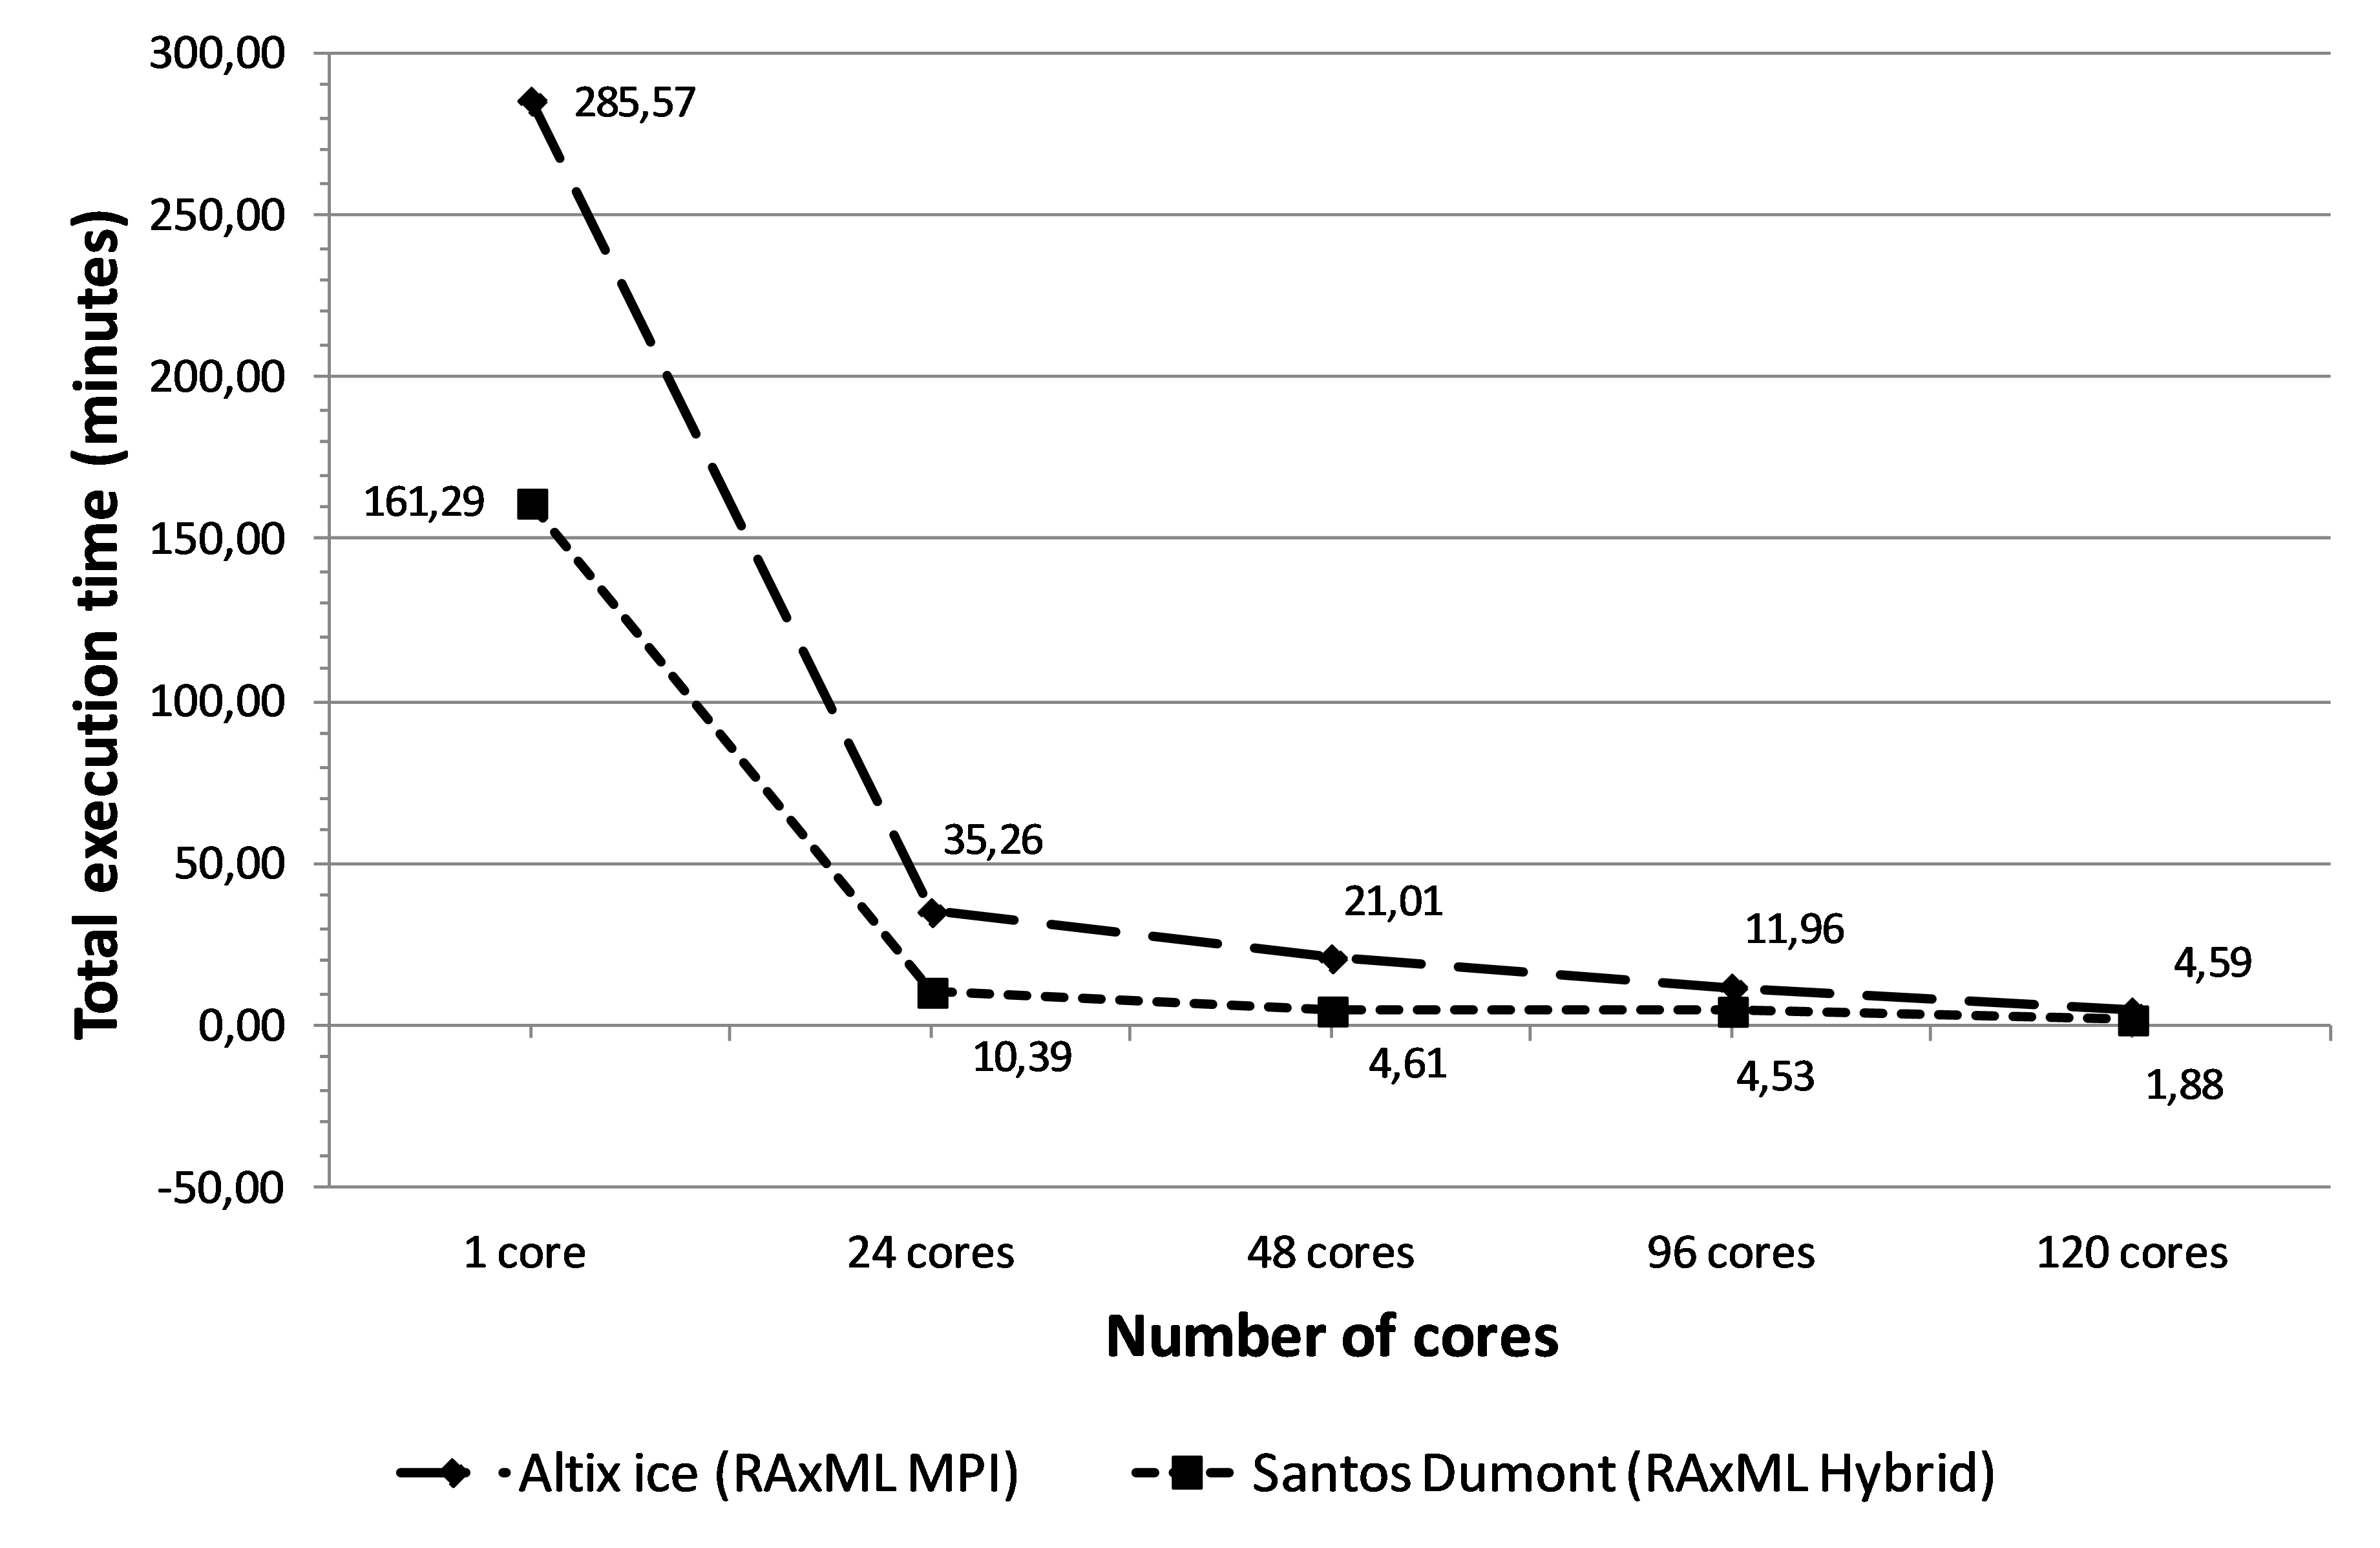
\includegraphics[width=0.6\textwidth]{imgs/raxmlscalabilityD5.png}
\vspace{-12px}
\caption{\system performance (scalability) results for \raxml MPI in Altix and \raxml Hybrid in SDumont for the superalignment D5}
\label{fig:raxmlscalabilityD5}
\end{figure}

\textit{3)The TET of \raxml MPI (Altix) and \raxml Hybrid (SDumont) using eight superalignments}. The executions of the \raxml versions used as input files eight superalignments, varying features of the number of taxa, number of amino acid, and size (KB). The parameters used for setting \raxml versions are JTT as the evolutionary model, GAMMA as the rate of the heterogeneity of the model, and 100 as the bootstrap value of replications. Figure~\ref{fig:raxmlTETAllD} presents the TET in hours of \raxml MPI and \raxml Hybrid in Altix using eight superalignments. The TET decreases, for all superalignments, when the \raxml parallel versions were executed. The eight superalignments files were categorized as Large (D1, D2), Medium (D3, D4, D7, D8), and Small (D5, D6). The versions \raxml MPI and \raxml Hybrid outperformed the versions \raxml HPC Serial and \raxml PThreads. With \raxml Hybrid, the TET of the largest file D1 was reduced from 820.60 hours (using one single core) to 30.10 hours (using 120 cores) and the TET of the smallest file D6 was reduced from 4.10 hours (using one single core) to 0.10 hours (using 120 cores). A relation was observed between the increment of the size of the superalignments files and the improvement of performance of approximately 90\% between 1 and 120 cores. D1: 2,091 KB and 96.33\%; D2: 1,260 KB and 95.99\%, D3: 792 KB and 95.78\%; D4: 553 KB and 95.47\%; D7: 168 KB and 95.63\%; D8: 157 KB and 94.75\%; D5: 95.83 KB and 97.83\%; D6: 72 KB and 97.50\%. These values indicate that parallelization benefits from larger files and that have more taxa and/or longer sequence lengths.

\begin{figure}[!htb]
\centering
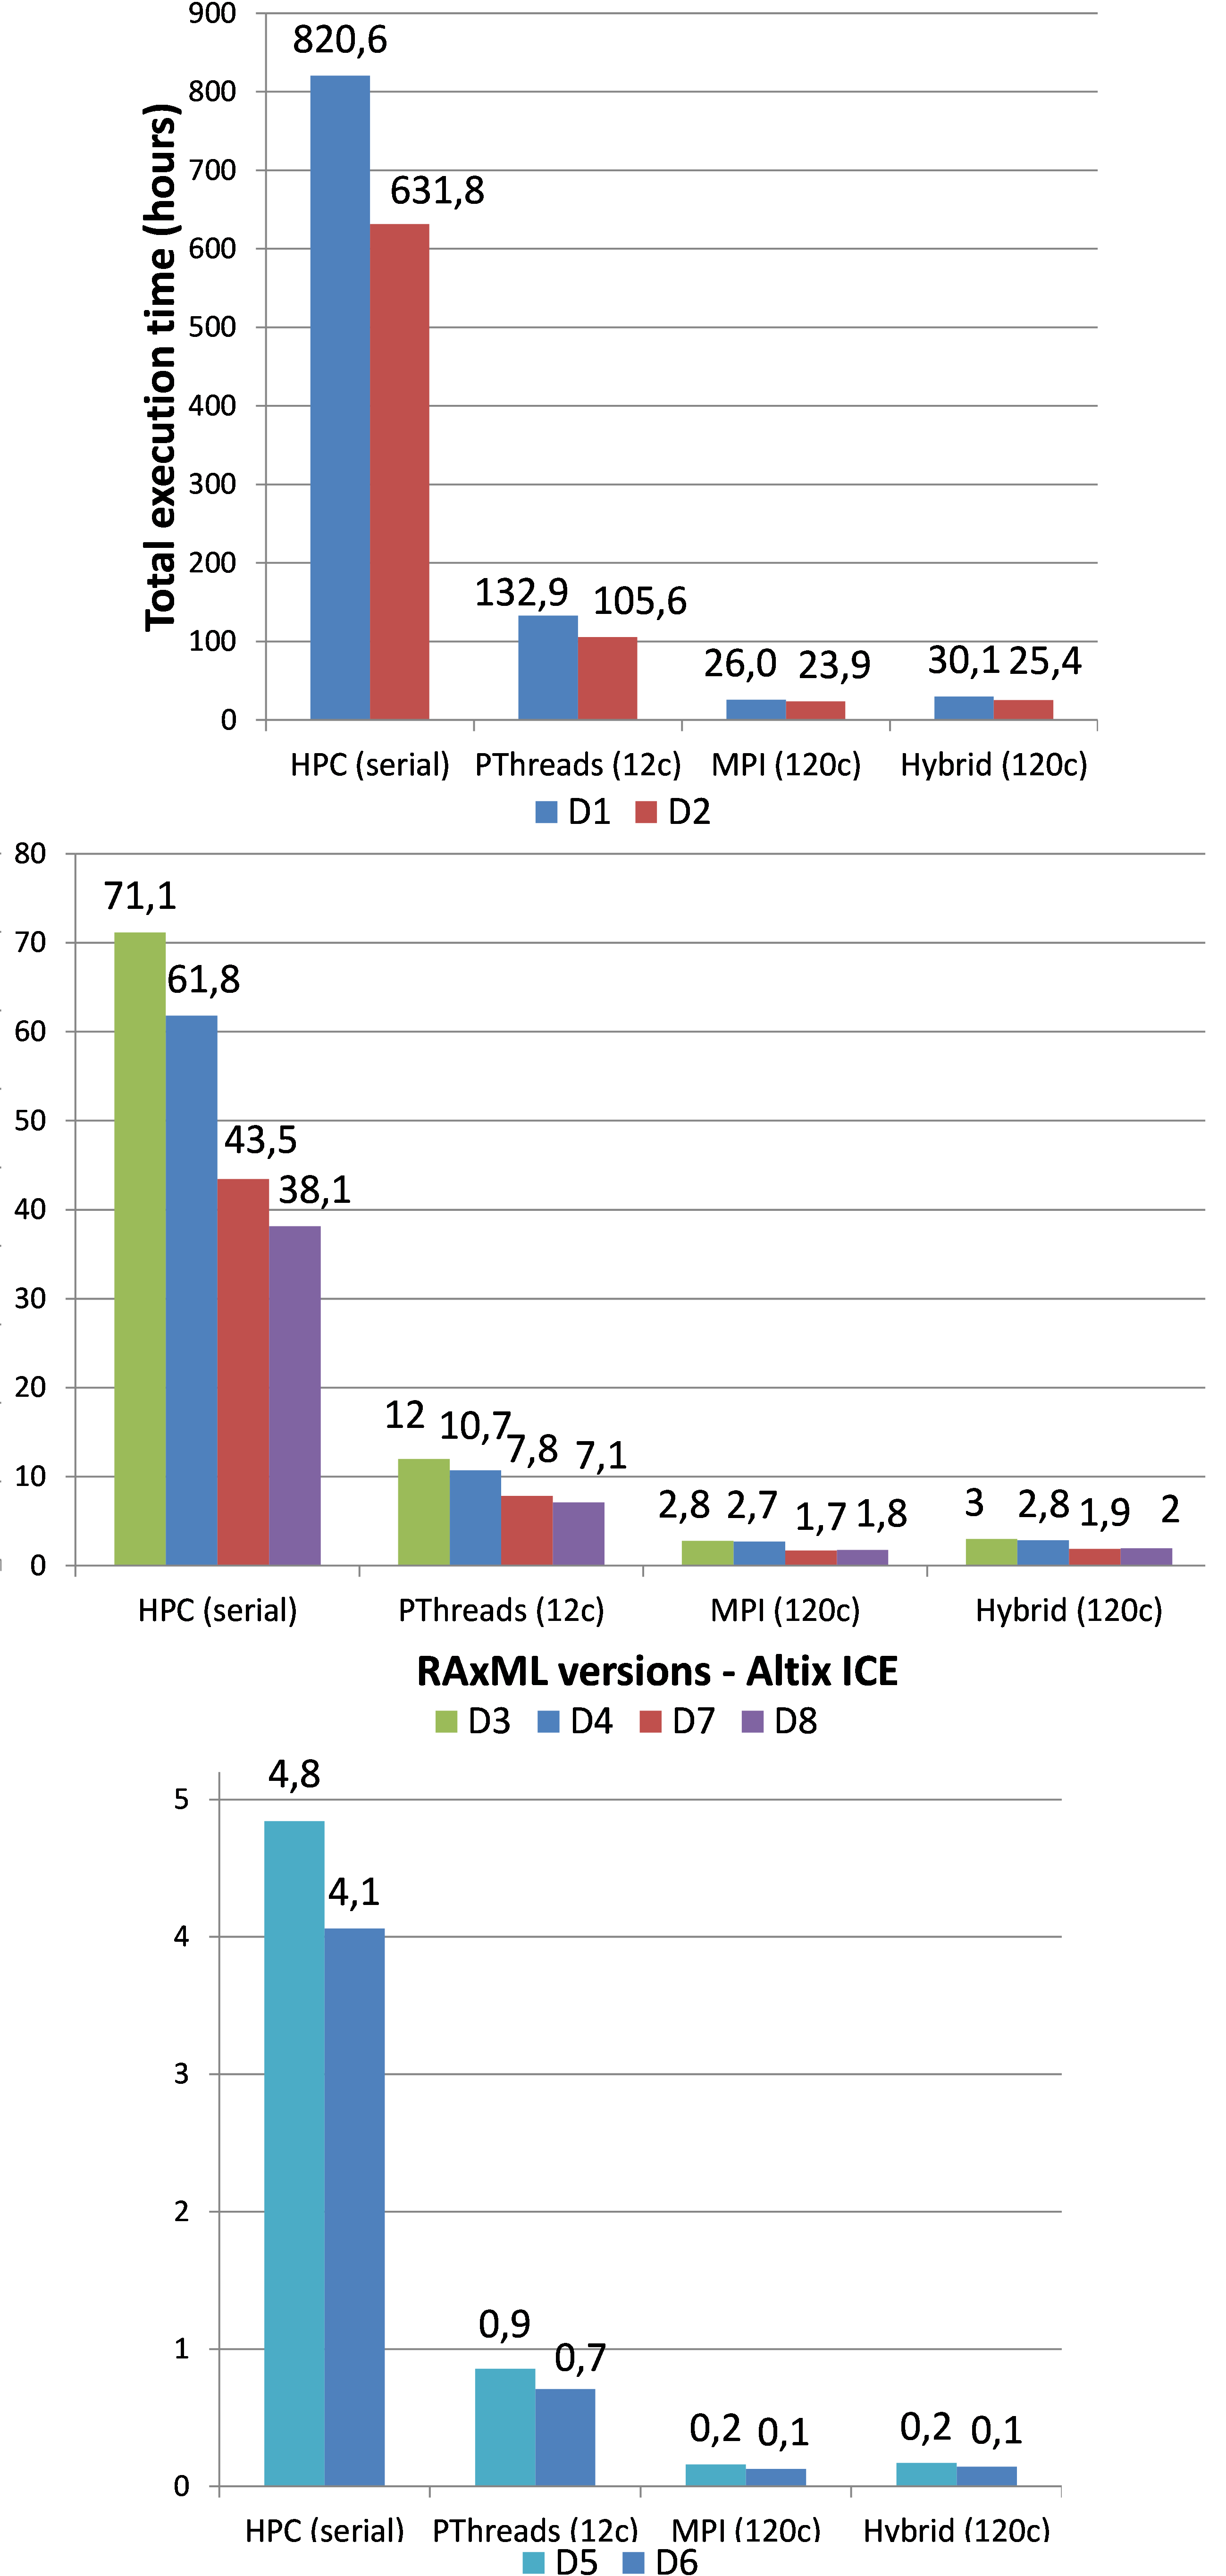
\includegraphics[width=0.6\textwidth]{imgs/raxmlTETAllD.png}
\vspace{-12px}
\caption{\system performance (TET) results for \raxml MPI and \raxml MPI in Altix for all eight superalignment}
\label{fig:raxmlTETAllD}
\end{figure}

\vspace{5px}
\noindent
\underline{\textbf{\sci}}, querying runtime the provenance database of SciCumulus allows to obtain the status of the \sci executions, which can be reported automatically as messages at the web interface \textit{e.g.} which activity is finished or if an error is presented. The arguments used as input files and parameters required to execute \sci through \system are: to upload the input file (alignment in FASTA format) and to fill the following options, input file type (\textit{e.g.} amino acid), e-mail, and output directory. Figure~\ref{fig:raxmlTETAllD} shows print messages at the final of each activity execution of \sci at \system, obtained by querying the SciCumulus provenance database. The activities that were successfully finished were printed in the web interface in green; on the other hand, those ones that reported an error in the execution were printed in red. 

\begin{figure}[!htb]
\centering
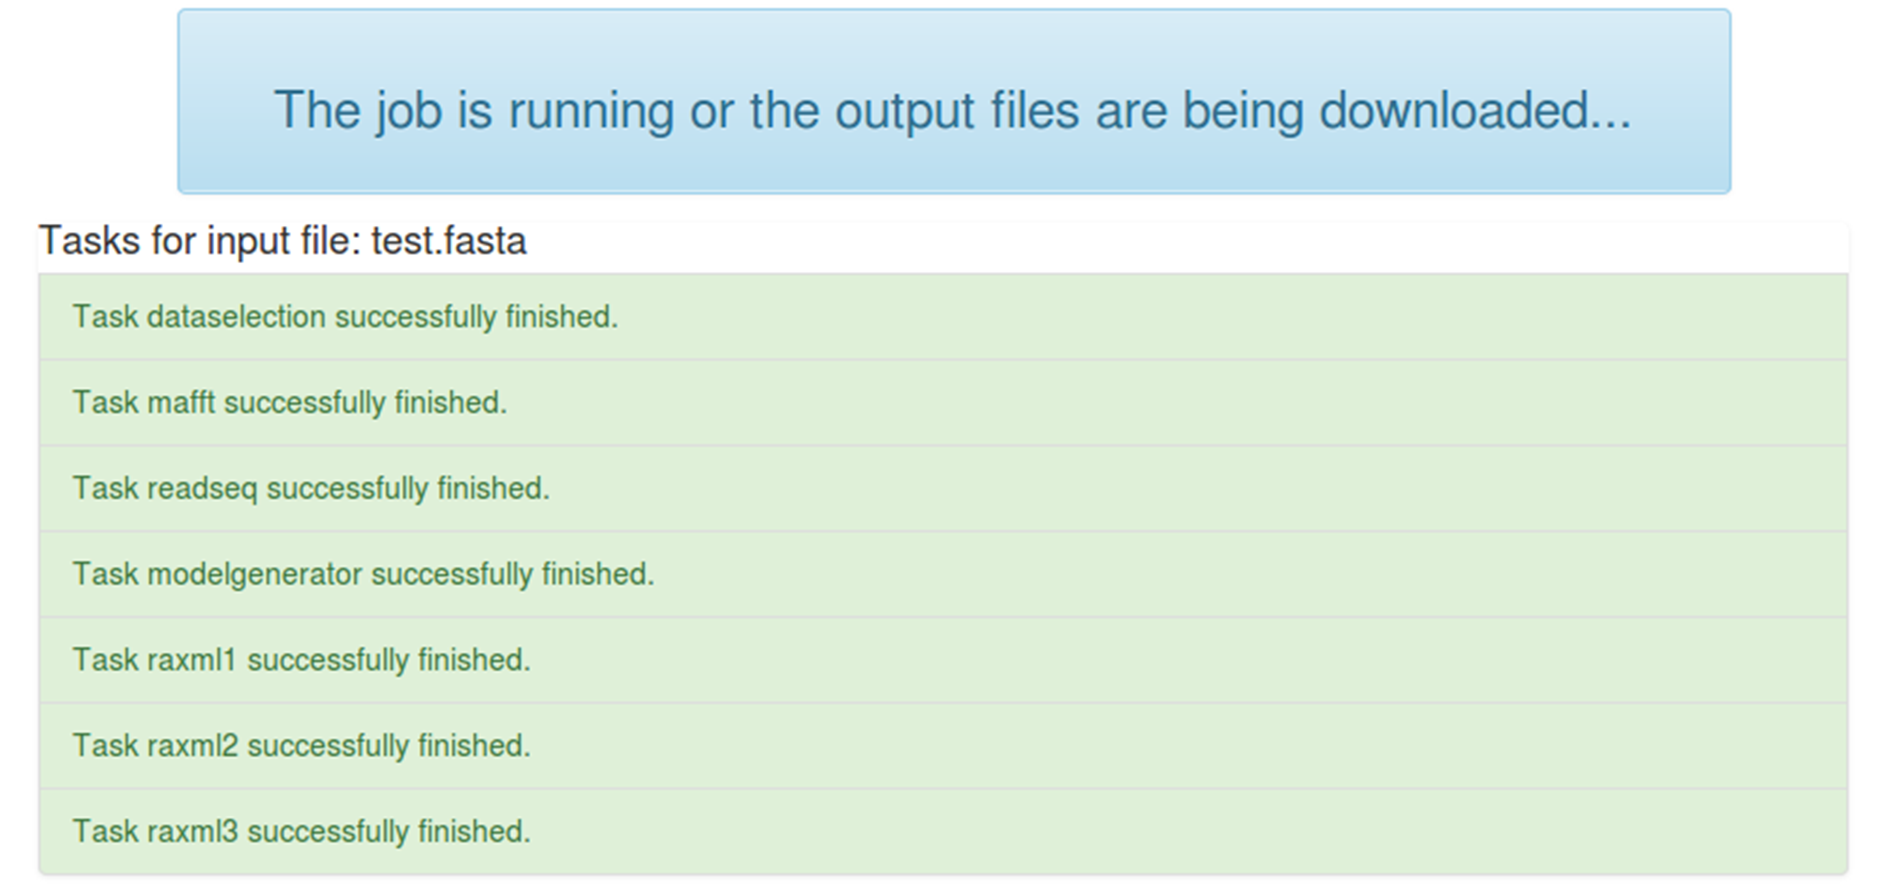
\includegraphics[width=0.6\textwidth]{imgs/sciphyoutputbioinfo.png}
\vspace{-12px}
\caption{\system output for \sci executions}
\label{fig:sciphyoutputbioinfo}
\end{figure}

We have evaluated the performance of the parallel execution of \sci in Altix. \sci was executed with 200 multifasta input files of amino acid sequences and three different configurations: on a single processor cluster (16 cores) through \system, on a single processor cluster (16 cores) directly at the cluster through CSGrid, and on three processor clusters (16 cores each) directly at the cluster through CSGrid. Figure~\ref{fig:sciphyTET} presents the TET in minutes of \sci, which presents the best performance with the third configuration \textit{i.e.} when it is executed directly at CSGrid with three clusters (in green). The TET was reduced from 374.75 minutes (using one single cluster through \system) to 180.19 minutes (using three clusters through CSGrid).

\begin{figure}[!htb]
\centering
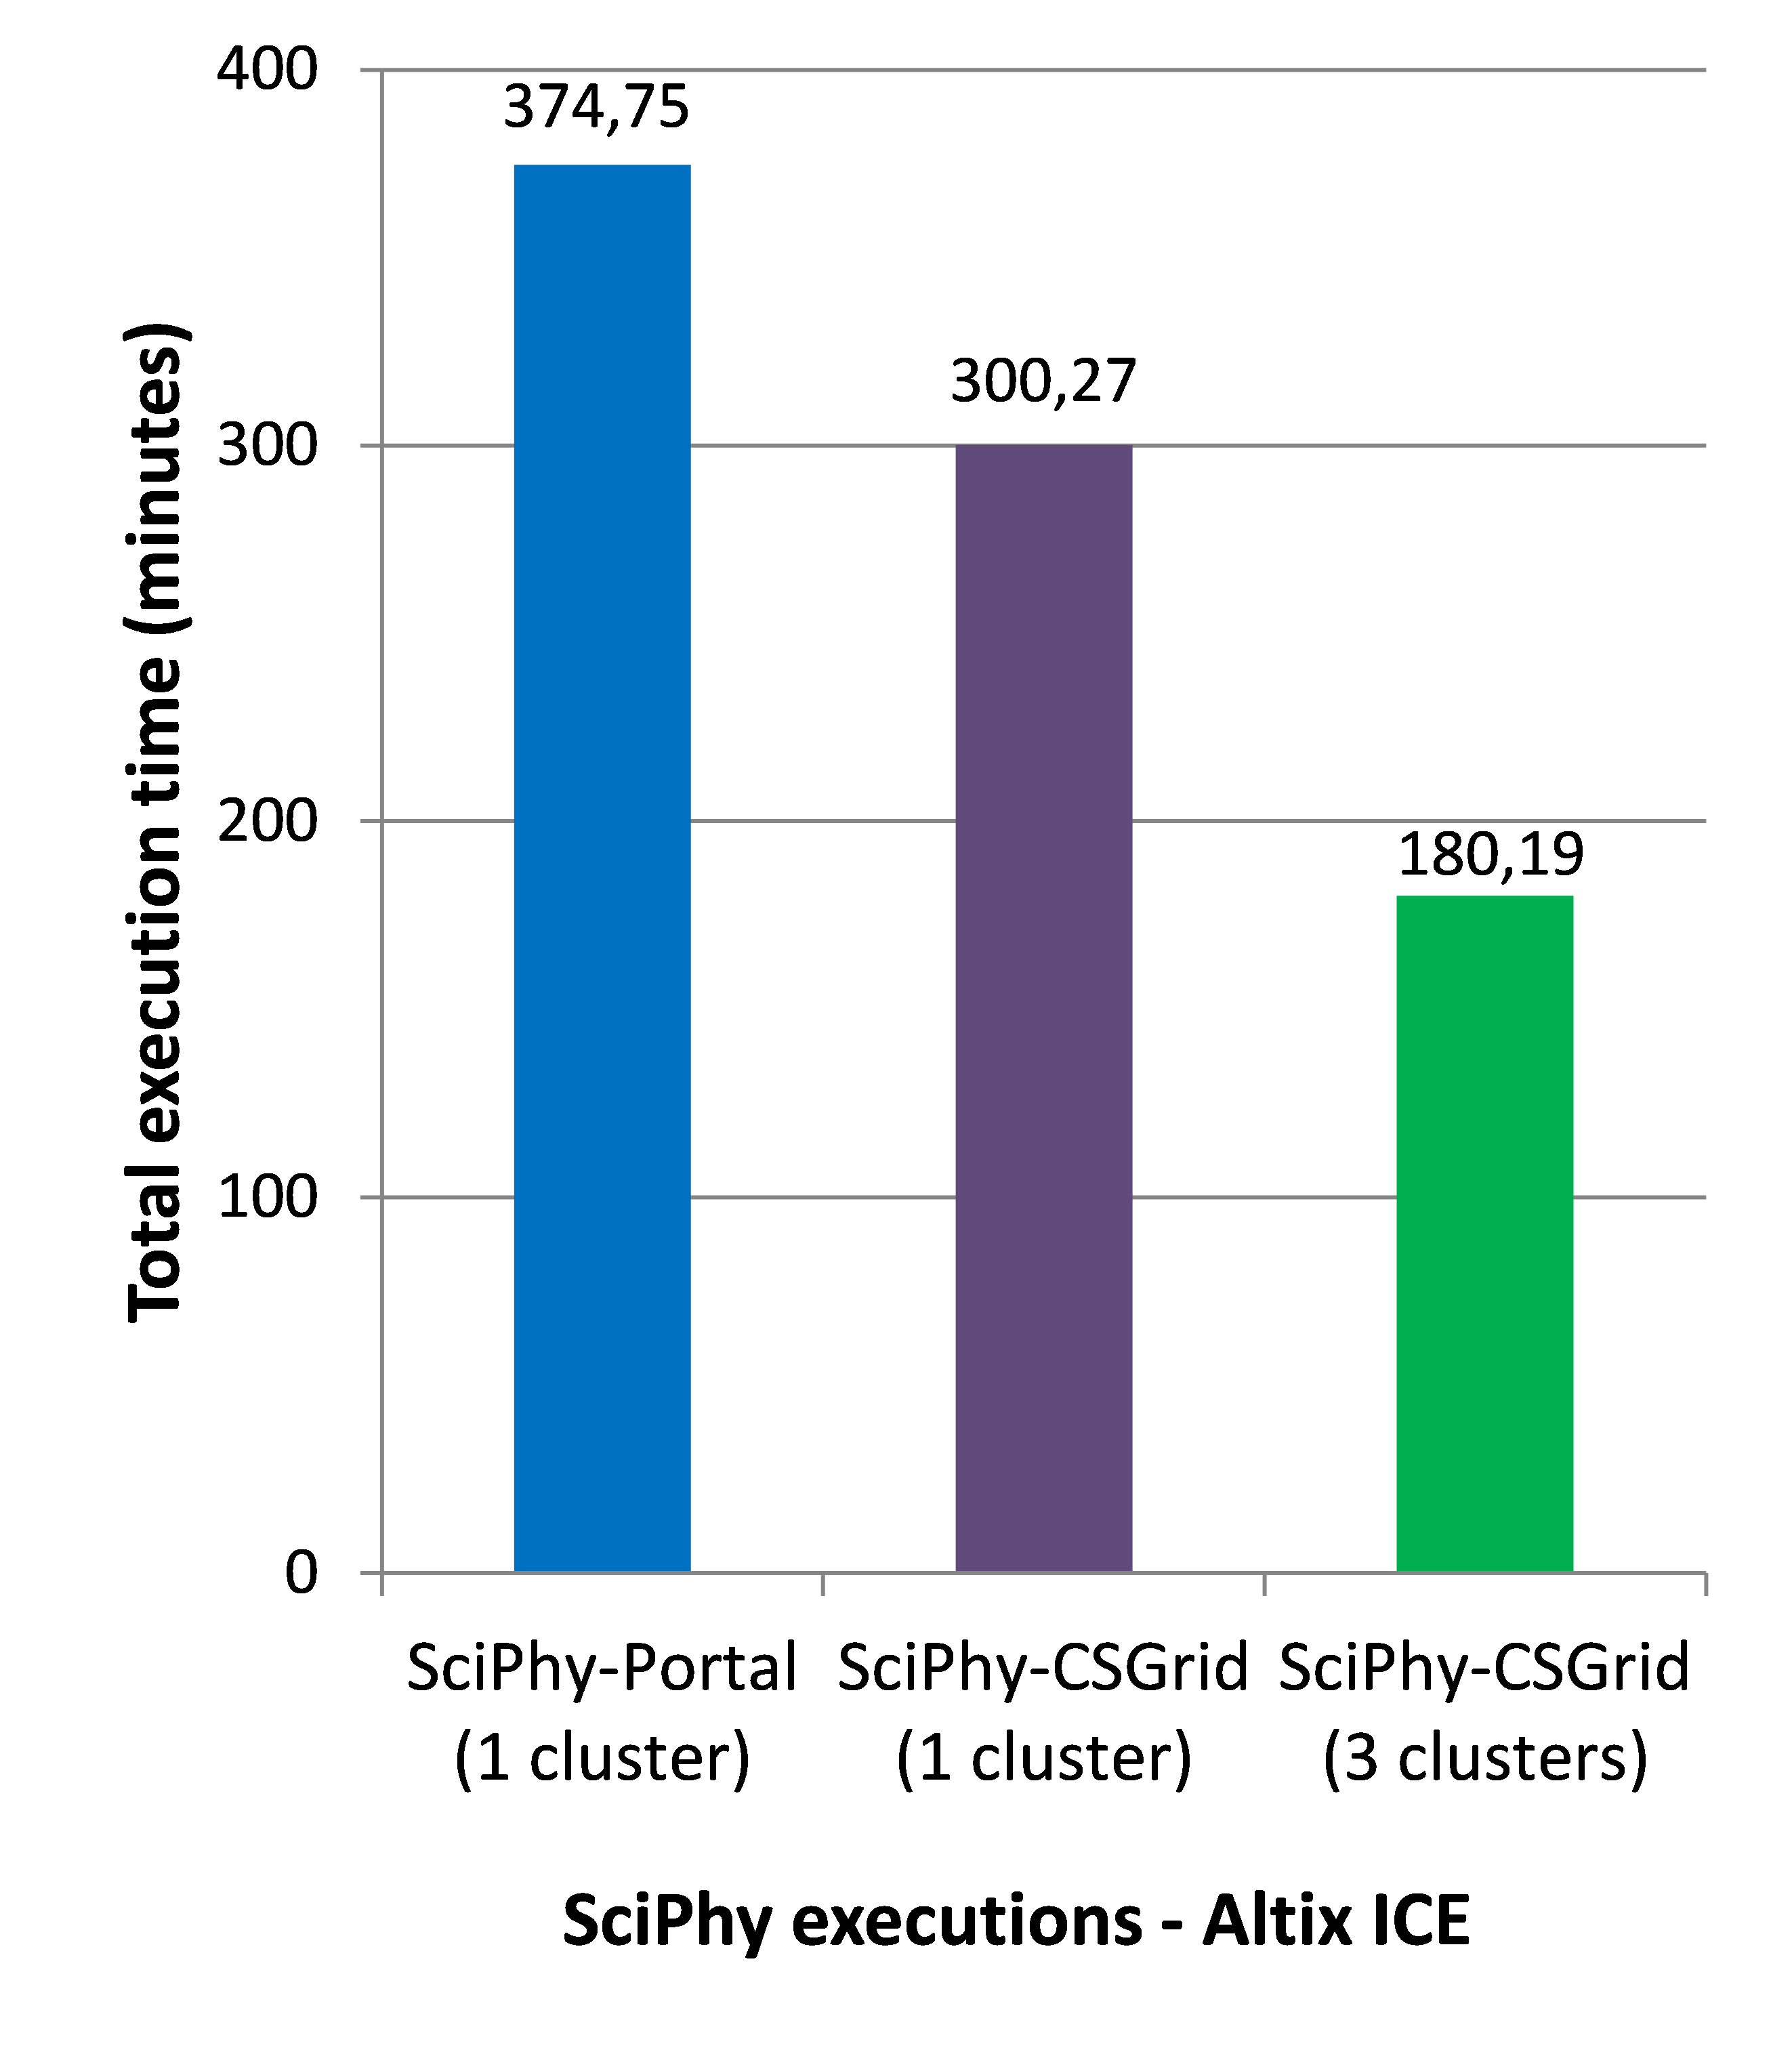
\includegraphics[width=0.6\textwidth]{imgs/sciphyTET.png}
\vspace{-12px}
\caption{\system output for \sci executions}
\label{fig:sciphyTET}
\end{figure}


\vspace{5px}
\noindent
\underline{\textbf{\swift}}, executions (resulting in 135 task executions) were performed in a cluster with 72 nodes, 16GB of RAM, and eight computing cores per node. The input data is formed by five genomes of bacteria completely annotated. The TET was based on three metrics: a sequential execution directly at the cluster (in red); a parallel execution directly at the cluster (in blue); and a parallel execution through CSGrid via \system (in green). Figure~\ref{fig:swiftgeckoTET} presents the TET in minutes of \swift, which presents the best performance with the second configuration \textit{i.e.} using a parallel execution directly at the cluster (in blue). The TET was reduced from 8.2 minutes (sequential execution directly at the cluster) to 4.23 minutes (parallel execution directly at the cluster). Experiments in Figure~\ref{fig:swiftgeckoTET} also shows that invoking a CSGrid function via \system introduces a small run-time overhead compared to parallel execution time. It is worth mentioning that \swift applications use an out-of-core strategy and are I/O intensive. Then, scalability could be improved by using higher throughput storage systems or more efficient data management strategies. Finally, the parallel execution through CSGrid via \system measures the time required for submission, execution, and file transference between CSGrid/SINAPAD and the cluster, which increment the time of response via \system.

\begin{figure}[!htb]
\centering
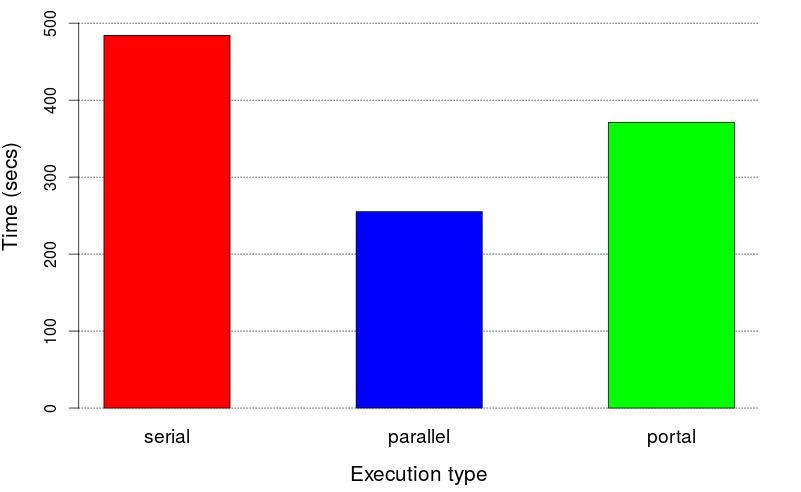
\includegraphics[width=0.6\textwidth]{imgs/swiftgeckoTET.png}
\vspace{-12px}
\caption{\system output for \swift executions}
\label{fig:swiftgeckoTET}
\end{figure}

\subsection{\system data analysis using machine learning}

The database of Bioinfo and provenance databases of the SWfMS were integrated into the statistical tools of Google Analytics. The information of jobs executed per month, jobs executed per applications, or session per country can be accessed to \system. Figure~\ref{fig:bioinfoTET} shows the TET in hours per applications executed until 01/11/2018. The applications most accessed were FragGeneScan, Align-m, and Phylip. Until 01/02/2019, the portal was accessed 2,812 times and 766 applications were executed.

\begin{figure}[!htb]
\centering
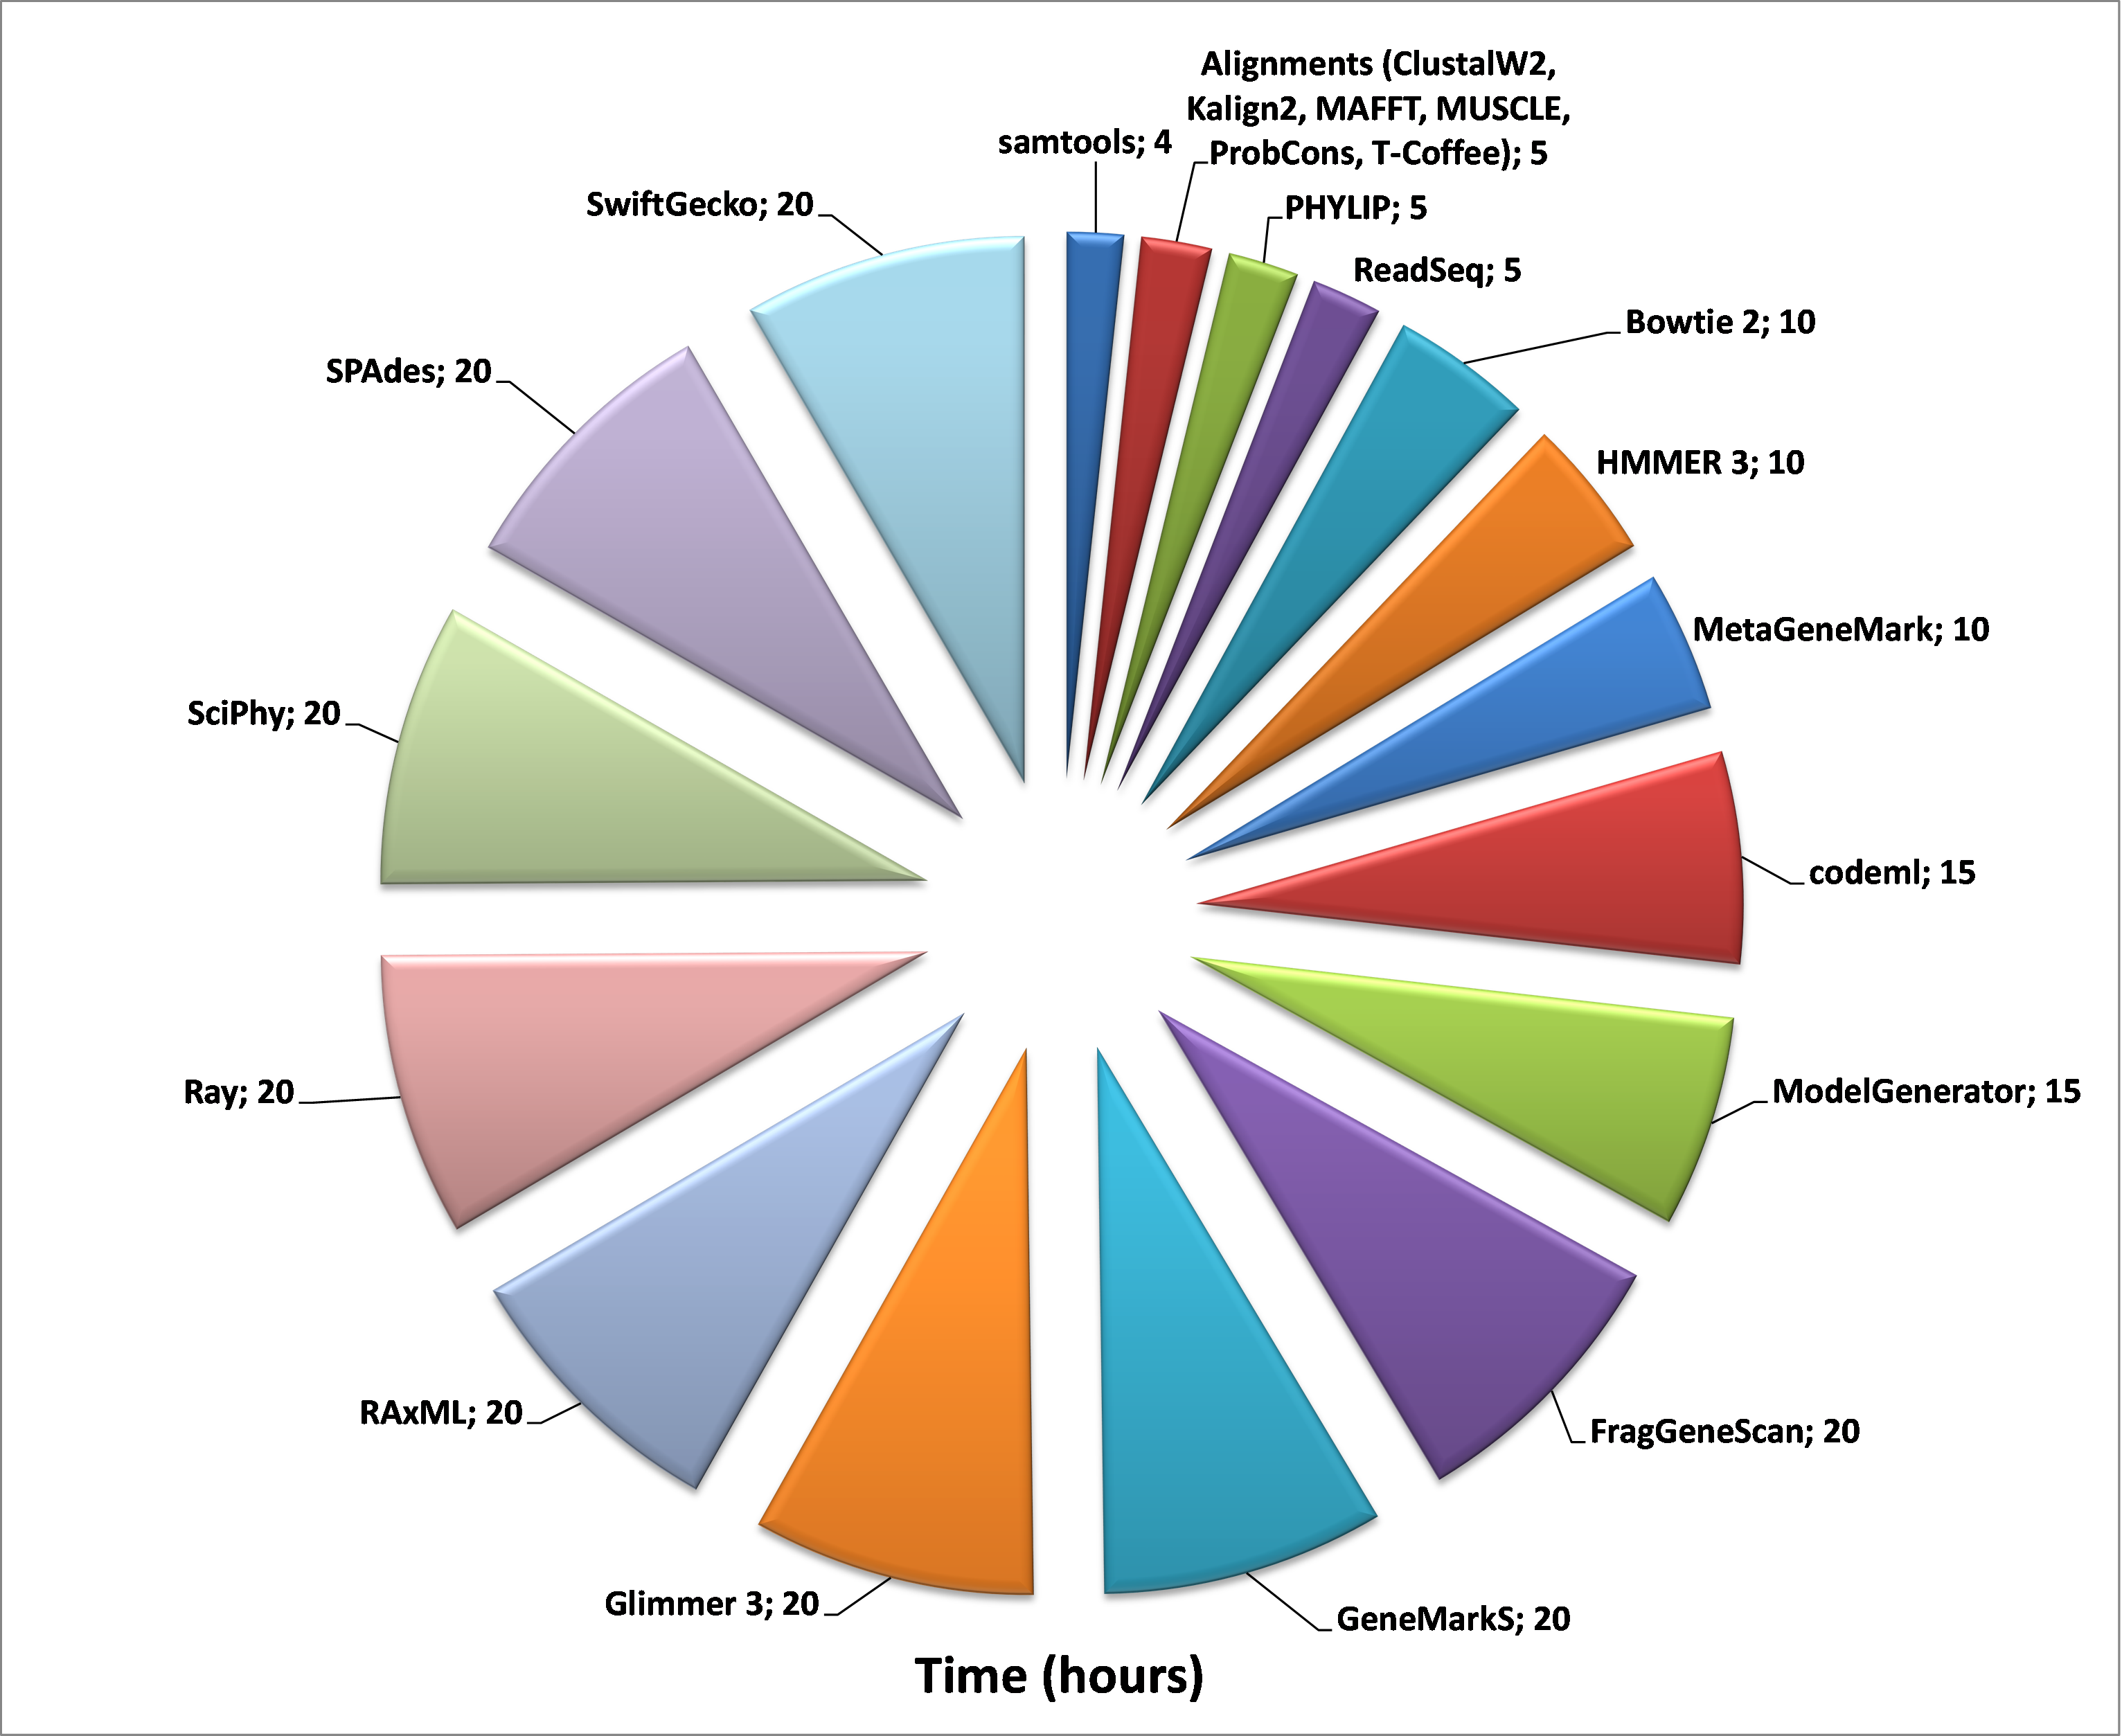
\includegraphics[width=0.6\textwidth]{imgs/bioinfoTET.png}
\vspace{-12px}
\caption{\system output for \swift executions}
\label{fig:bioinfoTET}
\end{figure}

An exploratory data analysis using classification trees was performed with the available data of the database of \system to infer knowledge about the most adequate computational resource to execute the applications. Data mining algorithms were used to discover patterns; we apply regression models with decision trees [22] using the Orange data mining tool for statistical analyses. Orange implements the core algorithm ID3 and employs a top-down, greedy search through the space of possible branches with no backtracking. Nevertheless, before generating the decision tree, we had to evaluate the statistics that each attribute used in the model (\textit{i.e.} threads, datasize, node attributes). The main idea of the attribute analysis is to identify potential problems with the chosen attributes and decide if an action needs to be taken that may require collecting more data. In Figure~\ref{fig:bioinfoTET}(a),(b),(c), we can state that there is no one dominant attribute value and the distribution is not even; and for our analyses, results indicate that attributes can be used in the predictions.

Figure~\ref{fig:bioinfoTET}(a) evaluates the threads attribute. We can observe that 75\% of the number of threads used was 24, from an interval of 24 to 240. Figure~\ref{fig:bioinfoTET}(b) shows that 75\% of data input presented size of 204 KB, from an interval of 3.2 to 610,000. Moreover, evaluating the node attribute in Figure~\ref{fig:bioinfoTET}(c), we observed that 75\% of the number of nodes used was 1, from an interval of 1 to 10. This information can assist users to distinguish outlier points to find anomalies or specific biological characteristics. By using these attributes to build estimation models, we can discover, using classification or regression algorithms, the relation of biological input data (size in KB) and the number of threads that can be used for the executions that generate maximum values of efficiency. Now we observed that the applications of \system consume low computational resources, which is due to the restriction for size and number of inputs assigned to the Projects of users.

\begin{figure}[!htb]
\centering
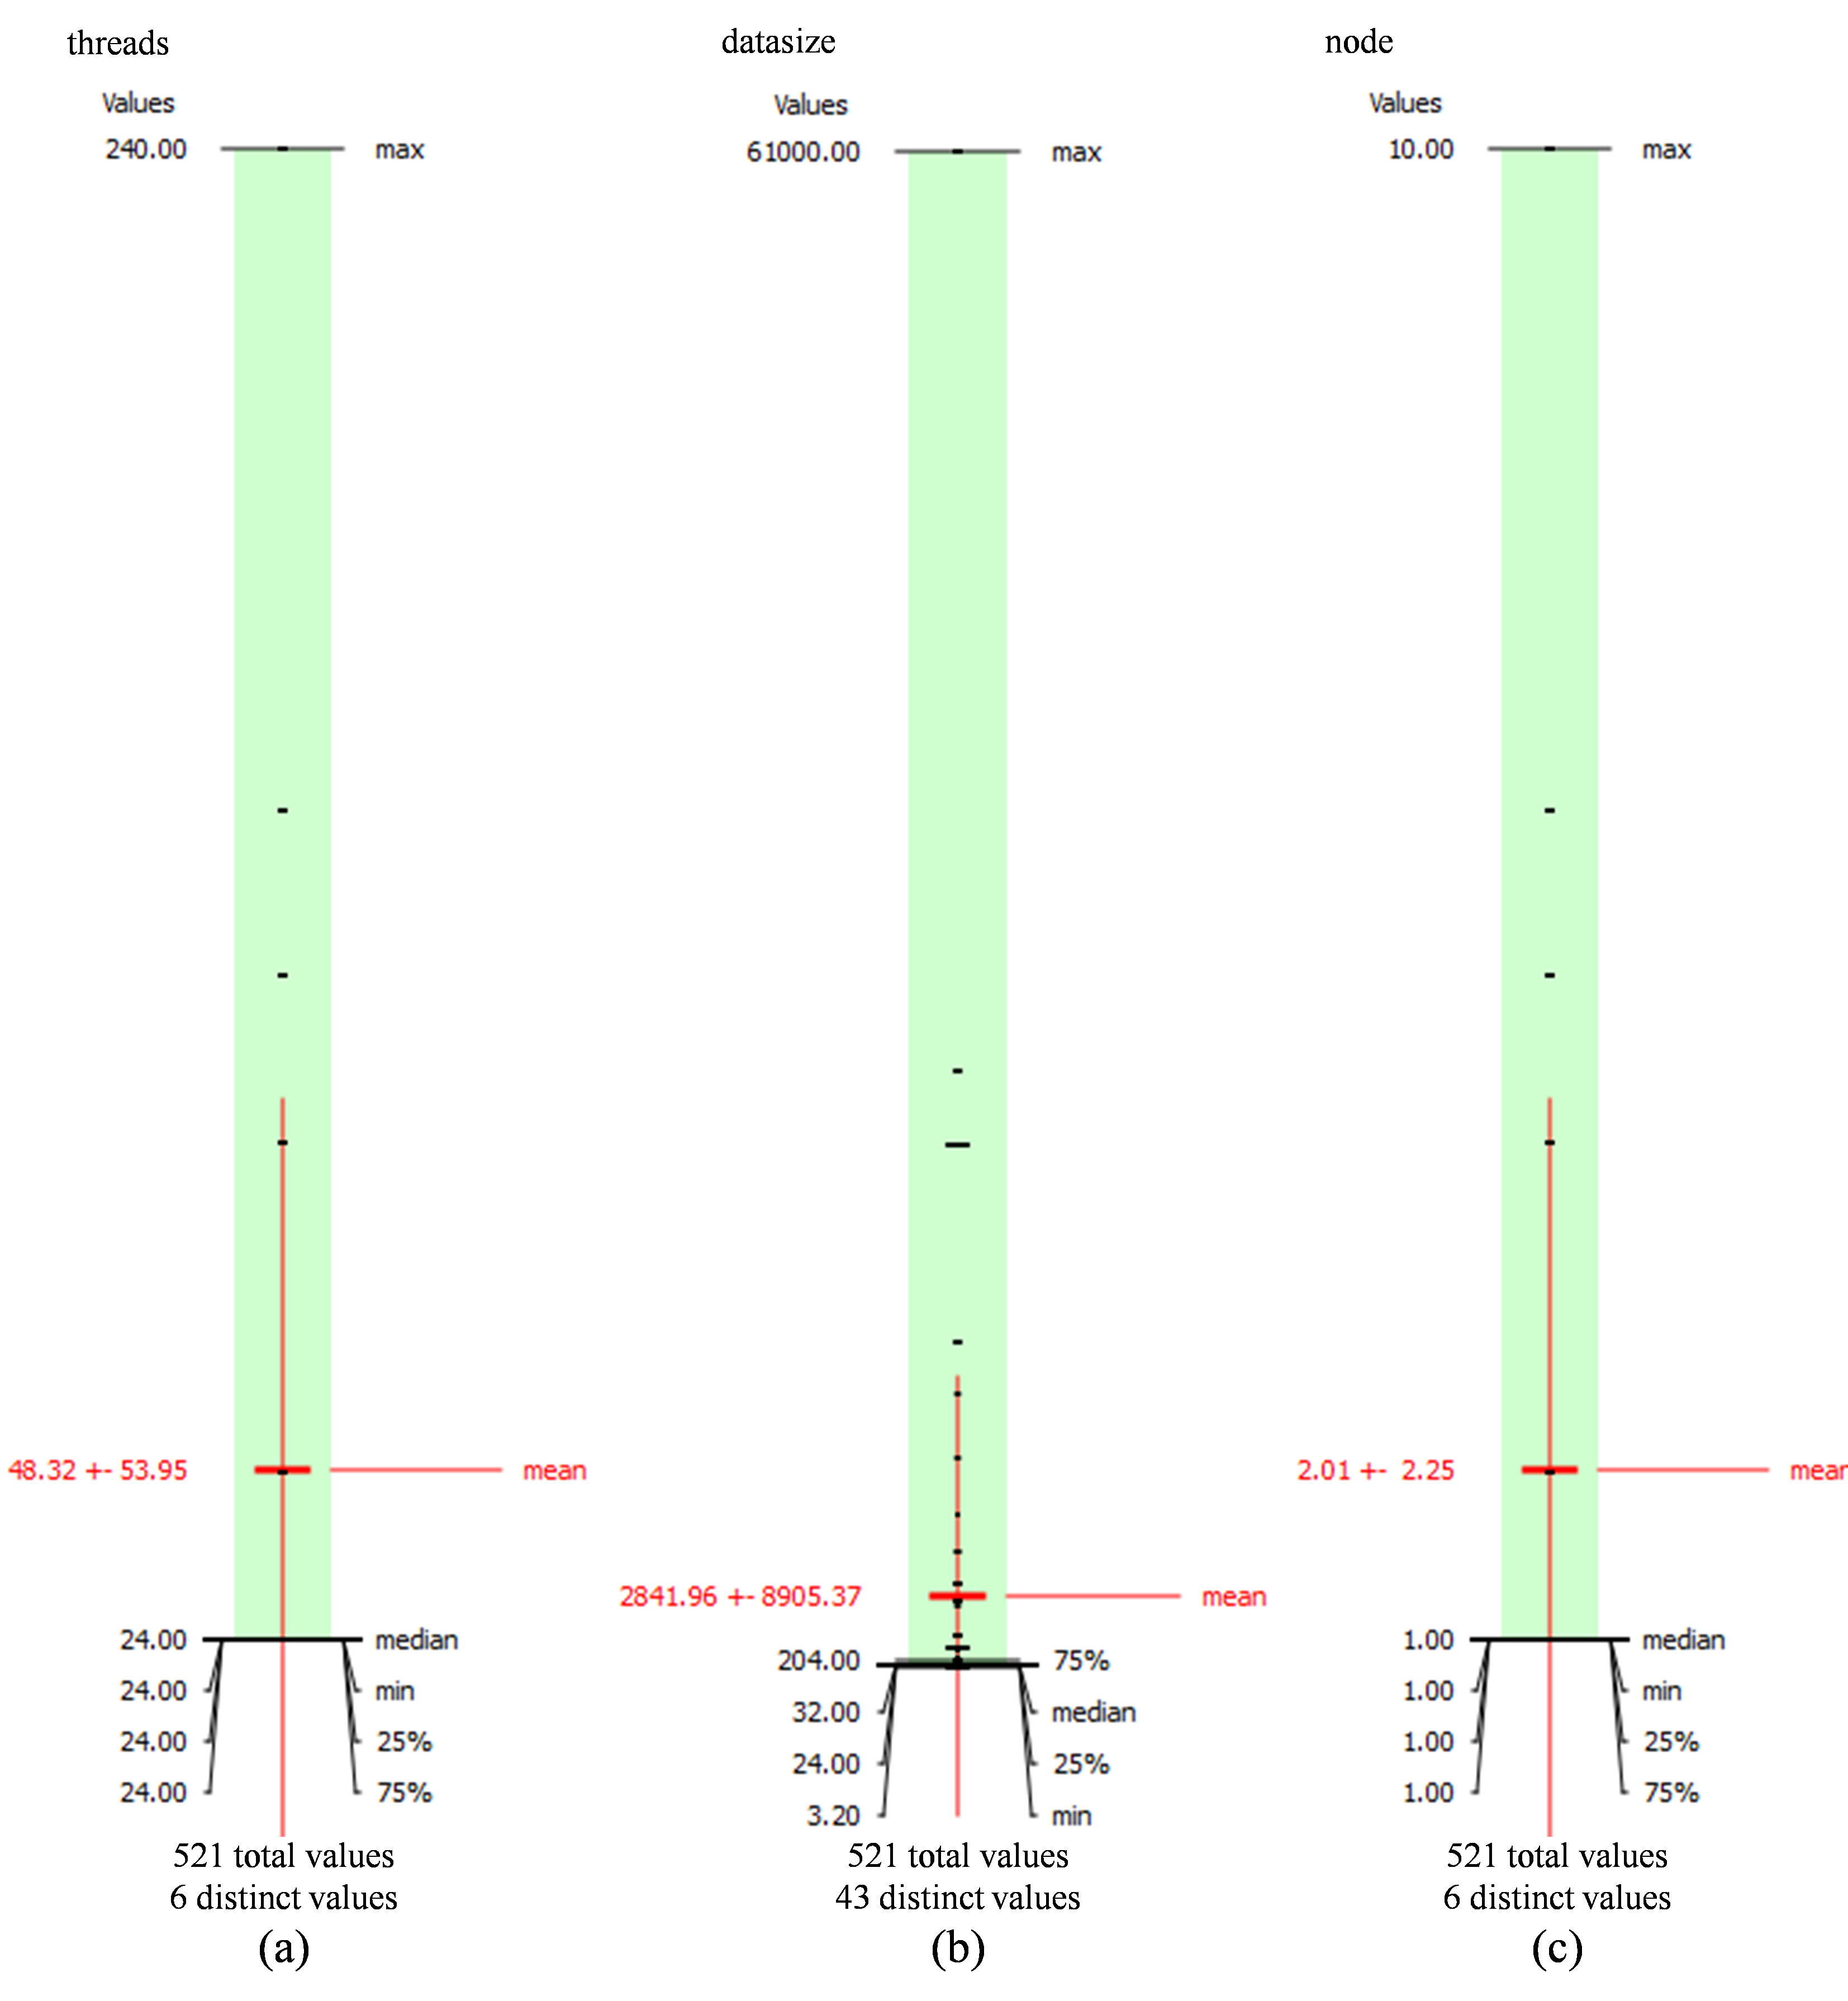
\includegraphics[width=0.7\textwidth]{imgs/mlattributes.png}
\vspace{-12px}
\caption{\system attribute statistics: (a) threads (number of threads), (b) datasize (data size of the alignment in KB), and (c) node (number of nodes)}
\label{fig:mlattributes}
\end{figure}

Figure~\ref{fig:mldecisiontree} presents the inferred rules for exploring the efficiency of the executions of applications at \system. In this analysis, we can state that the efficiency of computational resources of \system applications is determined by two parameters: the number of threads (threads), the size of the alignment in KB (datasize), and the number of nodes (node) \textit{i.e.} the combination of values of these three parameters defines the efficiency of the executions. 
For example, Figure~\ref{fig:mldecisiontree} presents that the efficiency that consumes the number of threads between 100 and 81 with less than 36,000 of size in KB of data size and will obtain, on average, 100 of efficiency. The machine-learning strategies appoint, for the actual scenario, that the best machine setup in a heterogeneous environment for executing applications presented at least 75\% of efficiency. However, results obtained are interesting and provide an idea about the behavior of application executions in HPC computational resources via \system, more refined experiments with more data must be reevaluated in future analyses. 

\begin{figure}[!htb]
\centering
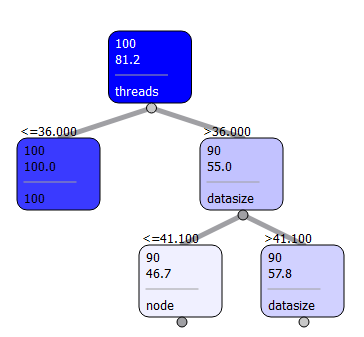
\includegraphics[width=0.6\textwidth]{imgs/mldecisiontree.png}
\vspace{-12px}
\caption{\system attribute statistics: (a) threads (number of threads), (b) datasize (data size of the alignment in KB), and (c) node (number of nodes)}
\label{fig:mldecisiontree}
\end{figure}

